\documentclass[oneside]{book}

\setcounter{secnumdepth}{4}

\setcounter{tocdepth}{4}

\usepackage{graphicx}
\usepackage[mathscr]{euscript}
\let\euscr\mathscr \let\mathscr\relax% just so we can load this and rsfs
\usepackage[scr]{rsfso}
\newcommand{\powerset}{\raisebox{.15\baselineskip}{\Large\ensuremath{\wp}}}

\usepackage{scalerel}

\usepackage{geometry}
\usepackage{listings}
\lstdefinestyle{lsstyle}{
	basicstyle=\ttfamily,
	basicstyle=\small,
	captionpos=b
}

\usepackage{hyperref}
\def\UrlBreaks{\do\/\do-}
\usepackage[bottom]{footmisc}

\usepackage{lipsum}

\usepackage{varwidth}
\usepackage{float}

\usepackage{cite}

\usepackage{graphicx}

\usepackage{subcaption,graphicx}

\usepackage{mathtools}


\lstset{style=lsstyle}

\usepackage{amsmath,systeme}

\DeclareMathOperator*{\argmax}{arg\,max}

\usepackage{verbatim}

\usepackage{courier}

\usepackage{hyperref}


\usepackage{url}

\usepackage{hyperref}

\geometry{a4paper}



\begin{document}



\begin{titlepage} 
	\noindent
	\begin{minipage}[t]{0.19\textwidth}
		\vspace{-4mm}{
\includegraphics[scale=1.15]{logo_unimib.pdf}}
	\end{minipage}
	\begin{minipage}[t]{0.81\textwidth}
	{
	{\textsc{Università degli Studi di Milano - Bicocca}} \\
	\textbf{Scuola di Scienze} \\
	\textbf{Dipartimento di Informatica, Sistemistica e Comunicazione} \\
	\textbf{Corso di laurea in Informatica} \\
	\par
	}
	\end{minipage}
	\vspace{40mm}
	
	\begin{center}{\LARGE{\textbf{Enhancing irony detection with affective information}\par}}
	\end{center}        
	\vspace{35mm}
	\noindent
	{\large \textbf{Relatore:} Prof.ssa Elisabetta Fersini} \\\\
	{\large \textbf{Co-Relatore:} Dott.ssa Debora Nozza} \\        
	\vspace{20mm}
	\begin{flushright}
		{\large \textbf{Relazione della prova finale di:}} \\
		\large{Gianluca Giudice} \\
		\large{Matricola 830694} 
	\end{flushright}
	\vspace{20mm}
	\begin{center}
		{\large{Anno Accademico 2019-2020}}
	\end{center}
\end{titlepage}
	
	

\tableofcontents


\chapter{Introduzione}

\section{Descrizione del problema}

La sentiment analysis è un campo dell'elaborazione del linguaggio naturale (NLP) che si occupa di costruire sistemi per l'analisi del testo, ha il fine di identificare e classificare l'informazione riguardo il sentimento e l'opinione espressa nello stesso. Si basa sui principali metodi di linguistica computazionale e di analisi testuale. L'analisi del sentiment è utilizzata in molteplici settori: dalla politica ai mercati azionari, dal marketing alla comunicazione, dall'analisi dei social media alla valutazione delle preferenze del consumatore. 

Il riconoscimento automatico dell'ironia nei contenuti generati da utenti, è uno dei compiti più complessi per quanto riguarda l'elaborazione del linguaggio naturale. Tuttavia è di fondamentale importanza per tutti i sistemi di sentiment analysis, in quanto facendo uso dell'ironia è possibile invertire completamente la polarità di una propria opinione, facendola passare da positiva a negativa e viceversa.
Diventa pertanto cruciale sviluppare dei sistemi che siano consapevoli del fenomeno e in grado di riconoscerlo.

L'ironia è un tema studiato in diverse discipline, come la linguistica, filosofia e psicologia, ma è difficile da definire formalmente, soprattutto per questo motivo ne è difficile il riconoscimento. Nonostante ciò ci sono basi teoriche che suggeriscono il ruolo importante della sfera emotiva nell'uso dell'ironia, quindi un fattore chiave per riconoscerlo. Con questo si intende anche un uso indiretto e non esplicito del carico emotivo in ciò che si vuole comunicare.

I social netowork in generale, e twitter nello specifico, sono ampiamente utilizzati come fonte di informazione per comprendere la web reputation di un brand, perciò si prestano bene per la sperimentazione di modelli computazionali per il riconoscimento dell'ironia, essendo di fatti una grande risorsa per quanto riguarda i dati testuali generati da utenti.


\section{Approccio al problema}
Si può considerare il riconoscimento dell'ironia come un problema di classificazione. Una frase potrà quindi essere classificata come appartenente alla classe ironica o non ironica. Si noti che per come viene approcciato il problema in questa tesi, l'ironia è considerata al pari del sarcasmo.

A questo scopo, la classificazione avviene mediante tecniche di machine learning (una branca dell'intelligenza artificiale). Nello specifico vengono creati dei modelli supervisionati tramite l'utilizzo di algoritmi, i quali fanno uso di una grande quantità di dati per estrarre dei pattern presenti in quest'ultimi.

Come già detto, twitter è una risorsa che fornisce moltissimi contenuti generati da utenti. Viene sfruttato questo aspetto collezionando i dati utilizzati dai modelli matematici, così da far apprendere la macchina con lo scopo di riconoscere l'ironia nel testo.

Il codice scritto in python, utilizzato per l'estrazione delle features, il training dei modelli, la creazione della matrice su cui è stata fatta PCA, oltre ai notebooks creati per l'analisi dei report e il risultato della PCA, è disponibile in questo repository\footnote{Irony detection repository: \url{www.github.com/gianlucagiudice/irony-detection}} su github.

\section{Sintesi dei risultati}
Il risultato degli esperimenti mostra come per il riconoscimento dell'ironia si ottengo i risultati migliori combinando tutte le features considerate. Inoltre le performance variano decisamente a seconda dell'algoritmo utilizzato per creare i classificatori. Nel caso preso in considerazione, l'algoritmo Support Vector Machine con un kernel lineare risulta essere il migliore tra quelli analizzati.

\chapter{Stato dell'arte}

\section*{Abstract}
L'ironia è una figura retorica molto importante, è uno strumento usato nella comunicazione in cui un individuo esprime l'opposto di ciò che realmente intende. Il riconoscimento automatico dell'ironia ha attirato l'attenzione nell'ambito natural language
processing (NLP) e machine learning (ML) così da dinvetare un ambito di ricerca. 

\section{Sarcasmo e sentiment analysis}
Facendo riferimento a \cite{survey4}, un'analisi dal punto di vista della linguistica computazionale sull'ironia, può fornire approfondimenti data-driven facendo luce riguardo i meccanismi nascosti nell'uso di questo fenomeno, potenzialmente migliorando la comprensione per quanto riguarda i processi mentali umani, la linguistica e la comunicazione. 

Tralasciando l'aspetto più filosofico, il riconoscimento dell'ironia ha implicazioni pratiche per quanto riguarda i sistemi di sentiment analysis, ed in effetti i modelli allo stato dell'arte in questo ambito, puntano proprio a portare benefici verso questi sistemi. Sentiment analysis vuol dire estrarre l'opinione di un individuo o della società riguardo un particolare evento o argomento. La presenza di ironia nei messaggi, è responsabile di errori nella classificazione in cui cadono i metodi allo stato dell'arte per la creazione di questi sistemi. Ciò avviene in quanto usando l'ironia viene invertita la polarità dell'opinione espressa nella frase, ingannando in questo modo gli approcci che non tengono in considerazione il fenomeno.

In questi anni i social network, soprattutto Twitter e Facebbok, hanno acquisito molta importanza in questo ambito, dal momento che gli individui condividono i propri pensieri, emozioni e opinioni su queste piattaforme. Di fatto, dato l'enorme contenuto di messaggi generati, questo è un esempio di Big Data. In diverse aree c'è un grande interesse nell'estrarre l'informazione riguardo l'opinione contenuta nei dati generati da utenti, così da conoscere, ad esempio, la reputazione relativa ad un prodotto piuttosto che l'opinione politica.

Per dare un'idea di quanto possano essere utili sistemi di questo tipo, come fatto notare nel survey \cite{survey1}, nel 2014 D. K. Tayal e altri \cite{political} hanno introdotto un sistema per riconoscere il sarcasmo e identificare la polarità espressa nei tweets politici. Il loro lavoro include la collezione del data set, data pre-processing e la classificazione. Attraverso un approccio supervisionato hanno concluso che da questi dati, comprendendo la componente sarcastica, è stato possibile fare una previsione sul risultato delle elezioni in modo efficiente.

\section{Difficoltà e problemi}
Come indicato nel survey \cite{survey3}, il riconoscimento dell'ironia è un compito complesso non solo per quanto riguarda le macchine, ma in alcuni casi anche per gli uomini. Questo è dovuto all'ambiguità intrinseca del sarcasmo.

In questi studi, il dataset è una componente fondamentale, dal momento che è necessario avere un dataset etichettato, la natura ambigua del sarcasmo viene risolta utilizzando la presenza di hashatg inseriti dagli utenti all'interno dei messaggi, ma senza questa informazione le frasi ironiche sono complicate da riconoscere.

\subsection{Ironia nel testo}
Per lavorare con il testo, è necessaria una rappresentazione numerica da dare in input ai vari algoritmi di classificazione. Un approccio unicamente bag-of-words tipicamente utilizzato nell'ambito NLP, non ottiene grandi performance in quanto usando il sarcasmo si possono esprimere opinioni negative facendo uso di parole positive. Tuttavia anche considerare altre features oltre a BOW può non risolvere completamente il problema, si pensi a quei messaggi molto corti in cui non è proprio possibile estrarre delle features.

Bisogna anche tenere in considerazione che nel testo è più difficile cogliere l'ironia rispetto che nel parlato, in quanto non si hanno a disposizioni features come il tono della voce, il linguaggio del corpo e le espressioni del volto. In questo ambito sono stati condotti degli studi da Tepperman e altri \cite{audio-sarcasm}, in cui si vuole riconoscere l'ironia nel parlato estraendo dallo spettro del suono features come l'intonazione, le pause ecc.


\subsection{Importanza del contesto}
Un altro aspetto importante, analizzato da Joshi e altri \cite{survey5} è il ruolo fondamentale del contesto quando si tratta di riconoscere il sarcasmo. Pur essendo questo un fattore chiave, Wallance in \cite{survey4} fa notare come non venga tenuto conto del contesto nella maggior parte dei modelli allo stato dell'arte.

Per contesto si intende l'informazione che va oltre il contenuto del testo di per sè. Oltre ad una conoscenza o semantica in generale, esistono altre informazioni legate al contesto come dettagli sull'autore (ad esempio vine tenuto conto del sesso in \cite{audio-sarcasm}), a chi viene rivolto il messaggio e l'ambito in generale.

In questo campo è stato condotto uno studio da Rajadesingan e altri \cite{scuba}, che hanno sviluppato il modello SCUBA (sarcasm using behavioral modeling). Basandosi su studi effettuati nel campo della psicologia e scienze comportamentali, per riconoscere il sarcasmo espresso da un utente, vengono analizzati i suoi tweets passati così da estrarre particolari caratteristiche comportamentali da usare come features per il classificatore. Un tale approccio è un esempio di modello che tiene conto del contesto.

 
\section{Linguistica del sarcasmo}
\subsection{Definizione formale}
Con lo scopo di meglio riconoscere il sarcasmo, nel survey \cite{survey2} ne viene data una definizione formale:
Una frase sarcastica può essere rappresentate da una sestupla $<S,\ H,\ C,\ u,\ P,\ P'>$ dove $S$ è chi parla, $H$ chi ascolta, $C$ il contesto, $u$ la frase, $P$ il senso letterale e $P'$ ciò che si vuole far intendere. 
Si noti come da questa definizione formale, emerge chiaramente che il contesto è un fattore chiave per cogliere il sarcasmo della frase.

Prendiamo come esempio, il cliente di un hotel che dice "Your room service was fantastic!" e il direttore è consapevole del fatto che il servizio sia stato peggiore rispetto al solito, utilizzando la rappresentazione 6-tupla si ha:


$\textbf{S}:$ Cliente

$\textbf{H}:$ Direttore

$\textbf{u}:$ "Your room service was fantastic!"

$\textbf{P}:$ Il servizio è stato \textit{ottimo}

$\textbf{P'}:$ Il servizio è stato \textit{pessimo}

\subsection{Tipi di sarcasmo}
Come fatto notare nel survey \cite{survey5}, esistono diversi tipi di sarcasmo. Camp nel suo lavoro \cite{tipi-sarcasmo} ne considera quattro diversi:
\begin{enumerate}
	\item \textbf{Propositional}: Un'affermazione come "Il tuo piano sembra fantastico" può essere interpretata come sarcastica o meno, dipende dal contesto.
	\item \textbf{Embedded}: Nella frase è presente una contraddizione intrinseca nella forma stessa delle parole utilizzate.
	
	Ad esempio considerando "Dato che si è rivelato così un bravo amico, ho deciso di smettere completamente di vederlo", emerge una chiara contraddizione.
	\item \textbf{Like-prefixed}: In questo tipo di sarcasmo viene implicitamente negato ciò che si afferma.
	
	Ad esempio "Come se la polizia troverà davvero l'assassino".
	\item \textbf{Illocutionary}: Sono casi in cui situazioni o azioni non relative al testo possono svelare il reale significato inteso dalla frase. 
	
	Ad esempio "Grazie per avermi tenuto la porta" può considerarsi una frase sarcastica solo conoscendo le circostanze (la porta non è stata realmente tenuta aperta).
	
\end{enumerate}


\section{Dataset utilizzati}
La qualità del dataset è un fattore cruciale per il riconoscimento dell'ironia/sarcasmo. In leteratura il più delle volte sono stati utilizzati dataset in lingua inglese, ma alcuni lavori sono stati fatti anche considerando lingue differenti, come l'italiano nel modello proposto da Barbieri e altri in \cite{sarcasm-ita}.

Come riportato in \cite{survey5}, anche la dimensioni dei messaggi cambia nei vari studi affrontati, andando a considerati testi brevi (tweets o  recensioni nei prodotti Amazon) o più lunghi (sottotitoli di una serie TV o conversazioni di un call center).

Nei dataset composti da testi brevi, cadono tutti quei contenuti generati da utenti sui social network ma non solo, si pensi ad esempio a recensioni nei prodotti di shop online. In particolare una piattaforma come Twitter si presta molto bene a studi riguardo il riconoscimento dell'ironia, dal momento che vengono messe a disposizioni delle API che rendono molto facile la creazione del dataset, oltre ad essere una piattaforma molto popolare ed utilizzata per esprimere opinioni.

Per effettuare gli studi è necessario avere un dataset etichettato.
Nel caso dei tweets sono state adottate due strategie diverse per assegnare ad ogni messaggio la classe di appartenenza (ironico / non ironico).

\begin{enumerate}
	\item \textbf{Crowdsourcing}: Consiste nell'annotare manualmente ogni tweet, questo compito è incaricato a delle persone che in alcuni casi \cite{crowd} sono proprio esperti del linguaggio. Chiaramente essendo necessario il coinvolgimento di risorse umane, questo processo è molto laborioso, e non si può pretendere di etichettare dataset di grandi dimensioni.
	\item \textbf{Self-taggin}: Questa tecnica si basa sull'uso degli hashtag. Assumendo che: se un utente utilizza l'hashtag \textit{\#scarcasm} o \textit{\#not}, allora ha l'intenzione di esprimere un messaggio ironico, questo semplifica nettamente la creazione del dataset, in quanto i messaggi ironici verranno etichettati come tali recuperando quei tweets che hanno al loro interno un determinato hashtag. In questo modo si ha il vantaggio di creare un dataset di grandi dimensioni con meno sforzo e in un tempo minore rispetto alla prima tecnica, in quanto può essere svolto automaticamente da una macchina. Inoltre un aspetto da non sottovalutare è che l'utente stesso viene tratto come il miglior giudice per annotare un suo messaggio come ironico o meno. Data la natura ambigua del sarcasmo, l'autore è colui che meglio conosce la vera natura del messaggio.
	
\end{enumerate}

Inoltre per quanto riguarda la tecnica crowdsourcing, Joshi e altri \cite{survey5} hanno fatto notare l'influenza di differenti culture quando si tratta di etichettare i messaggi ironici. Infatti i loro risultati mostrano come, dato un dataset americano da far annotare sia a persone americane che indiane, i secondi concordavano maggiormente rispetto agli americani, inoltre gli indiani avevano difficoltà riguardo studi o entità a loro sconosciuti (trattandosi di un dataset americano).

Si noti inoltre che l'ironia è un fenomeno non molto frequente nel linguaggio, questo si riflette in un dataset non bilanciato, aspetto da tenere conto se si vuole adottare la migliore tecnica di classificazione. Questa problematica è stata affrontata da Liu e altri in \cite{imbalance} facendo uso di tecniche ensemble.


\section{Approcci adottati}
Nello stato dell'arte il riconoscimento dell'ironia viene formulato come un task di classificazione, quindi dato un tweet riconoscerlo come ironico o non ironico. Esistono  diversi approcci per questo tipo di problema, anche se la maggior parte dello stato dell'arte utilizza modelli supervisionati. Come primo passo è necessaria una fase di pre-processing. I dati generati da utenti presentano infatti del rumore, e questa fase è un passo preliminare fondamentale per riconoscere l'ironia. Il pre-processing consiste sostanzialmente nell'effettuare la tokenizzazione, rimuovere le stop-words, stemmatizzare e lemmatizzare. Si può inoltre adottare una tecnica di POS tagging per associare ad ogni parola l'informazione riguardo la parte del linguaggio a cui essa appartiene, come ad esempio il nome, aggettivo, nome ecc.

\subsection{Approcci rule based}
Tra gli approcci rule-based troviamo il modello proposto da Maynard e altri in \cite{hashtag}, dove il sentiment dell'hashtag utilizzato in un messaggio, viene considerato come un fattore chiave per riconoscere il sarcasmo. Pertanto un tweet viene classificato come sarcastico nel caso in cui il sentiment dell'hashtag non è coerente con il resto del tweet.

Un ulteriore approccio non supervisionato è stato proposto da Bharti e altri \cite{parsing-tree} in cui vengono usate due regole di classificazione:
La prima consiste nel creare un parsing tree basato sul lessico a partire dalla frase, vengono quindi individuate le espressioni che trasportano del sentiment. Se una locuzione negativa è presente in una frase positiva, allora la frase è classificata come sarcastica. La seconda regola di decisione è costituita da un algoritmo che mira a catturare le espressioni iperboliche individuando interiezioni (come "wow") e intensificatori (come "assolutamente").

Riloff e altri \cite{rilof}, presentano un approccio rule-based in cui, tramite l'utilizzo di un algoritmo, viene considerata la struttura sintattica del tweet. Vengono quindi cercati all'interno della frase i verbi con sentiment positivo e espressioni negative. La regola di decisione consiste nel classificare un tweet come sarcastico nel caso in cui sia presente questa contraddizione tra sentiment.


\subsection{Insieme delle features}
La scelta delle features è un altro compito importante per riconoscere correttamente l'ironia.
In letteratura sono state utilizzate diverse features, un elenco esaustivo è riportato da \cite{survey5}. La maggior parte degli approcci utilizza bag-of-words, ma in aggiunta a questo sono state utilizzate ulteriori features:

González-Ibánez e altri \cite{gonzalez} utilizzano il sentiment basandosi sul lessico, oltre che considerare le particelle pragmatiche come le emoticons, e il fatto di citare altri utenti all'interno di un messaggio;
Nel lavoro di Farias e altri \cite{farias} vengono utilizzati dei lessici come AFINN e SentiWordNet per estrarre caratteristiche riguardo il contenuto emotivo delle parole;
Reyes e altri \cite{reyes} introducono features riguardo l'ambiguità nella frase, facendo riferimento ad ambiguità nella struttura, nella semantica, tra morfologia e sintassi, oltre a considerare features che danno una misura di quanto sia inusuale la relazione semantica tra le parole; Liebrecht e altri \cite{gram} considerano bigrammi e trigrammi come features, dove per n-gramma si fa riferimento ad una sottosequenza di n elementi in una specifica sequenza;
Barbieri e altri \cite{sarcasm-ita} sfruttano dei lessici per utilizzare come features l'intensità del sentiment dei nomi, verbi, aggettivi e avverbi. Calcolando quindi il valore minimo, il valore massimo, e il gap tra questi. Inoltre viene considerato il numero massimo/minimo/medio di sinonimi per le parole presenti in uno specifico documento.


L'utilizzo di nuove features, come riportato da \cite{survey1}, può migliorare le performance dei classificatori, ma  è necessario uno studio più approfondito riguardo features come la semantica, espressioni iperboliche, punteggiatura ecc. 

\subsection{Approcci semi supervisionati}
Tra gli approcci semi supervisionati troviamo l'esempio dell'algoritmo introdotto da Davidov e altri \cite{davidov}, con lo scopo di  riconoscere il sarcasmo nei tweets e recensioni di prodotti Amazon. Tale approccio consiste nell'identificare dei pattern presenti nelle frasi, dopodiché questi pattern vengono automaticamente estratti dal dataset e la feature principale consiste nel vettore in cui viene riportata la presenza (o assenza) del pattern all'interno del testo in input.

\subsection{Approcci supervisionati}
L'approccio generale consiste nel creare modelli supervisionati, dove partendo dal dataset, si passa per una fase di pre-processing. Dopodiché vengono estratte delle features dal testo. Si usano quindi i classici algoritmi di machine learning (SVM, Naive Bayes, Decision tree) per effettuare il training dei modelli, vengono poi testati con la tecnica cross-validation per valutare il più performante.

Come esempio di modelli supervisionati possiamo trovare il lavoro svolto da Farías e altri \cite{farias} in cui vengono estratte alcune delle features elencate sopra, considerate altre ulteriori caratteristiche e creati classificatori con gli algoritmi Decision Tree e Support Vector Machine. Reyes e altri \cite{reyes} utilizzano gli algoritmi Naive Bayes e Decision Tree, mentre Barbieri e altri \cite{sarcasm-ita} usano binary Logistic Regression.
Ulteriori approcci supervisionati, come nel caso di Fersini e altri \cite{fersini}, sfruttano tecniche ensemble, nello specifico Bayesian Model Averaging (BMA), in cui diversi classificatori vengono combinati considerando ognuno di questi durante la classificazione, in questo modo si è in grado di ottenere una classificazione più affidabile.



\subsection{Deep Learning}
Come fatto notare in \cite{survey5}, le tecniche basate su architetture deep learning hanno acquisto popolarità nel campo NLP, di conseguenza alcuni approcci si basano su questi modelli per il riconoscimento dell'ironia.

Un esempio è il modello proposto da Joshi \cite{embeddings} in cui viene utilizzata la similarità tra gli embeddings delle parole per cercare di migliorare il riconoscimento dell'ironia. Un ulteriore esempio è il modello proposto da Bharti e altri \cite{deep-learning} che consiste in una combinazioni di Convolutional Neural Network, Recurrent Neural Network e Deep Neural Network, dal loro lavoro emerge un miglioramento delle performance rispetto ad altri modelli allo stato dell'arte. Zhang e altri \cite{zang} approcciano il riconoscimento dell'ironia come un task di transfer learning, in cui vengono usati modelli pre-trained per sfruttare la conoscenza acquisita riguardo il sentiment. Il loro lavoro si concentra nel cogliere incongruenza implicite presenti nei messaggi, senza basarsi su espressioni esplicite. I risultati mostrano come questo modello supera le performance rispetto altri modelli allo state dell'arte.

\section{Conclusioni}
Il riconoscimento dell'ironia è una delle sfide principali nell'ambito della sentiment analysis, e negli ultimi anni ha acquisito man mano più importanza. Si tratta di un campo nel data mining che richiede maggiori approfondimenti.

Per etichettare il dataset vengono utilizzate tecniche manuali o l'uso di hashtag. Il problema viene approcciato come un task di classificazione e si usano approcci rule-based, semi-supervisionati e supervisionati, sono state inoltre adottate tecniche di deep learning, le quali sembrano essere la strada giusta per lavori futuri.

Un ruolo chiave nel riconoscimento dell'ironia è svolto dal contesto. Tali informazioni fanno parte di ciò che non viene scritto direttamente all'interno della frase. Alcuni studi sono stati svolti a riguardo, tenendo in considerazione tweets passati di un determinato utente, piuttosto che mediante tecniche di transferred learning che incorporano informazioni acquisite riguardo al sentiment nei modelli pre-trained.

Ad oggi i modelli allo stato dell'arte hanno performance peggiori nel riconoscere l'ironia rispetto agli umani. Come fatto notare da Wallace in \cite{survey4}, il problema principale degli esistenti modelli di machine learning, può essere una poca considerazione del contesto.

Wallace fa notare come tutti i modelli allo stato dell'arte approcciano il task di riconoscimento dell'ironia/sarcasmo come un problema di classificazione. Non vi sono approcci che hanno lo scopo di determinare il tipo di sarcasmo, piuttosto che ricostruire il significato latente della frase.

\chapter{Sistema realizzato}

\section{Descrizione del sistema proposto}
In questa tesi, per riconoscere l'ironia nel testo, vengono proposti dei modelli supervisionati di machine learning.
Il dataset a disposizione è una collezione di tweets. Partendo da questi dati si utilizzano tecniche di pre-processing che consistono nel pulire il testo di partenza e prepararlo per essere dato in input ai diversi algoritmi per creare i classificatori. Inoltre si estraggono delle features da ogni messaggio, le quali più sono discriminanti nel riconoscimento dell'ironia, meglio distinguono la classe di appartenenza.

Il dataset viene diviso in due parti: training set e test set. La prima ha dimensione decisamente maggiore e viene utilizzata per far apprendere uno specifico classificatore, l'altra per testarlo. Questo è importante in quanto un determinato modello dovrà riconoscere l'ironia in un generico documento e non solo tra quelli a disposizione. Si noti che entrambe le porzioni di dati sono composte sia dal testo già codificato e processato che le features estratte, hanno solo scopi diversi quando si tratta di creare il classificatore. 

Vengono quindi creati vari modelli fornendo in input il dataset di training, con lo scopo di far apprendere la macchina. Avendo costruito più classificatori che utilizzano diversi algoritmi per apprendere dai dati, è possibile confrontarne le performance per valutare il migliore tra tutti, ovvero quello che meglio distingue tra documenti ironici e non ironici.

\begin{figure}
	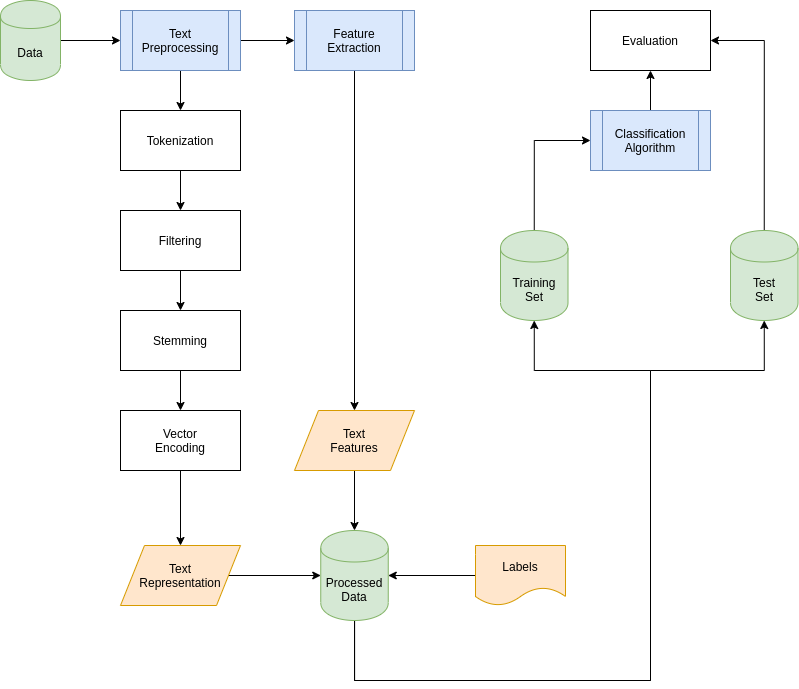
\includegraphics[width=\linewidth]{assets/Workflow.png}
	\caption{Workflow.}
	\label{fig:workflow}
\end{figure}


\clearpage

\section{Dati in input}
Trattandosi di modelli supervisionati, per il training dei classificatori è necessaria una collezione di testi (in questo caso tweet) con le relative etichette associate ad ogni documento. Il testo e le labels compongono il dataset, questo aspetto è cruciale in quanto una volta aver opportunamente processato i tweets, saranno proprio questi i dati forniti in input al classificatore. La fase di training ha lo scopo di far apprendere al classificatore, così facendo sarà poi in grado di riconoscere l'ironia in testi che non ha mai visto prima.


\begin{table}[h!]
	\centering
	\begin{tabular}[t]{lr}
		\hline
		\textbf{Tweet} & \textbf{Label assocaita}\\
		\hline
		Lorem ipsum dolor sit amet, consectetur adipiscing elit & ironico     \\
		Cras ornare turpis ut odio finibus, viverra porta felis lobortis & ironico \\
		Suspendisse in ex a felis porta convallis & non ironico \\
		Nam laoreet, lacus at ullamcorper iaculis, id interdum nisl elit nec elit. & non ironico \\
		
		\hline
	\end{tabular}
	\caption{Esempio di dataset a disposizione.}
\end{table}%




\section{Rappresentazione del testo}
Il corpora a disposizione è definito "crudo" e non può essere direttamente utilizzato per la fase di training. Prima è necessario codificare il testo per ottenere una rappresentazione numerica da dare in input all'algoritmo. A questo scopo sono state utilizzate due diverse tecniche: BOW e Transformer.

\subsection{Rappresentazione Bag-of-word}
La prima tecnica di rappresentazione utilizzata è boolean bag-of-words.
Il testo viene codificato come una matrice booleana composta dai documenti sulle righe e i tokens sulle colonne. I tokens sono tutte quelle parole appartenenti ad un dizionario costruito a partire dal corpora, tutte le operazioni eseguite sono spiegate di seguito.

\subsubsection{Tokenization}
La tokenizzazione è un passo preliminare per l'elaborazione computazionale del testo. Tokenizzare vuol dire dividere le sequenze di caratteri in unità minime di analisi dette "token". Un approccio potrebbe essere considerare un token come una sequenza di caratteri delimitata da spazi, tuttavia una tale definizione lascia spazio a numerose eccezzione, come ad esempio la presenza di punteggiatura. Per questa operaziona viene utilizzata la libreria
nltkl \cite{nltk} in grado di gestire correttamente tutti questi casi limite, oltre a poter sfruttare una Twitter-aware tokenization adattandosi quindi bene al dominio in questione.

\begin{figure}[!h]
	\centering
	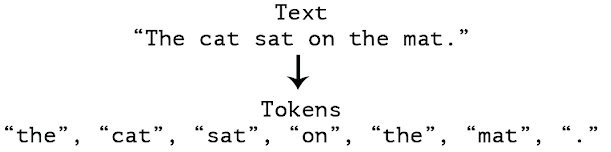
\includegraphics[width=9cm]{assets/text-to-tokens.jpg}
	\caption{Text tokenization.}
	\label{fig:tokenization}
\end{figure}


\pagebreak

I vari tokens estratti vengono convertiti in lowercase e sono considerati validi solo se in match con il pattern regex \texttt{[a-z]+}. Così facendo non si considerano gli hashtag, la punteggiatura, le emoticons e tutto ciò che non è considerato come parola.

Il risultato ottenuto è una lista di tokens validi contenuti in ogni tweet:

\begin{table}[h!]
	\centering
	\begin{tabular}[t]{l|l}
		\hline
		\textbf{Tweet} & \textbf{Tokens validi}\\
		\hline
		Lorem ipsum dolor sit amet, consectetur adipiscing elit				& [$t_1$, $t_2$, $t_3$, $t_4$, $t_5$] \\
		Cras ornare turpis ut odio finibus, viverra porta felis lobortis 	& [$t_6$, $t_7$, $t_1$, $t_8$, $t_9$, $t_4$] \\
		Suspendisse in ex a felis porta convallis							& [$t_{10}$, $t_6$, $t_{11}$, $t_{12}$] \\
		Nam laoreet, lacus at ullamcorper iaculis.							& [$t_{13}$, $t_{14}$, $t_8$, $t_{15}$]\\
		
		\hline
	\end{tabular}
	\caption{Esempio di tokens associati ad ogni tweet.}
\end{table}
\noindent
Da qui si crea l'insieme di tokens univoci a partire dai tokens presenti in ogni tweet.

\subsubsection{Filtering}
\label{section:filtering}
L'insieme di termini univoci ottenuto è filtrato in base ai seguenti criteri:
\begin{itemize}
	\item \textbf{Occorrenza minimia}:
		Viene fissato un valore di threshold (per gli esperimenti eseguiti è 10) e si scartano tutte quelle parole che compaiono tra tutti i documenti meno del valore scelto. 
	\item \textbf{Stopwords + RT}:	
		Vengono scartate tutte le parole più comuni che sono generalmente presenti in una frase. Queste sono un insieme predefinito contenente parole come gli articoli, proposizioni, pronomi e verbi ausiliari.
		
		Es: $\{a,\ the,\ of,\ is,\ into,\ it,\ ...\}$
		
		Dato il dominio preso in considerazione, è possibile che un utente compia l'operazione di reTweet. Questo è codificato nei messaggi dall'abbreviazione \emph{"rt"}. Non ritenendolo un aspetto rilevante per il riconoscimento dell'ironia, viene anch'essa considerata una stopwords, e di conseguenza non trattato come token valido.
	
		
	\item \textbf{Irony e Ironic}:
	Essendo il dataset a disposizione etichettato mediante la tecnica self-tagging (\autoref{chap:self-taggin}), è presente l'hashtag \emph{\#irony} in tutti i tweet ironici. Pertanto nell'insieme dei tokens validi verranno escluse le parole \emph{irony} e \emph{ironic}, così da non avere un bias nei dati sotto questo aspetto. Nel caso contrario i dati usati per creare i modelli avrebbero a disposizione una componente che ben distingue i tweet ironici, ma che nella realtà non sarebbe presente, in quanto non è decisamente corretto assumere che ogni testo ironico contenga una delle due parole.
	
	
\end{itemize}

\subsubsection{Stemming}
Lo stemming è il processo di riduzione della forma flessa di una parola alla sua forma radice.


\begin{figure}[!h]
	\centering
	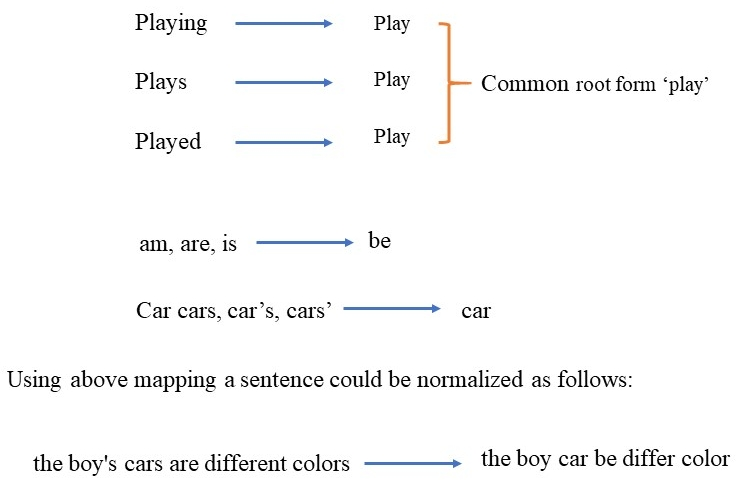
\includegraphics[width=11cm]{assets/stemming.jpg}

	\caption[Caption for LOF]{Words stemming.\footnotemark}
	\label{fig:stemming}
\end{figure}


\footnotetext{Fonte: \url{www.datacamp.com/community/tutorials/stemming-lemmatization-python}.}


Con questa tecnica è possibile ridurre il numero di tokens, dal momento che, ad esempio, le stesse parole con suffisso diverso verranno mappate nella medesima radice. Inoltre non è necessario che una parola dopo il processo di stemming venga trasformata in un'altra di senso compiuto, quello che conta è la semantica del token.


\subsubsection{Vector encoding}
Arrivati a questo punto, l'insieme delle parole ottenute costituisce il dizionario del corpora. Si procede costruendo una matrice booleana composta dai tweets sulle righe e le parole del dizionario sulle colonne.\\

Sia $D = \{w_1,\ w_2, ...,\ w_m\}$ il dizionario individuato dall'insieme delle $m$ parole univoche.

Sia $T_i = \{t_{i0}\ ,t_{i1},\ ...,\ t_{ik}\}, \ 1 \leq i \leq n$, l'i-esimo tweet composto dai $k$ tokens opportunamente stemmatizzati presenti nello stesso.\\
Viene definita la matrice $M_{n,m}$:
\[
M[i,j] =
\begin{cases}
1 & \text{se}\ w_j \in T_i\\
0 & \text{altrimenti}
\end{cases}
\ \;t.c\ 1\leq i\leq n,\ 1 \leq j \leq m
\]


\subsection{Rappresentazione mediante Transformer}
Nell'ambito dei modelli di deep learning, per Transformer si intende un particolare tipo di architettura di rete neurale. Questi modelli hanno il vantaggio di essere parallelizzabili, ciò comporta una diminuzione di tempo per la fase di training. Inoltre fanno uso di alcuni particolari meccanismi  per meglio comprendere la semantica della frase\cite{transformer}. Uno dei meccanismi principali viene chiamato "attenzione", considerando l'analogia con quello che è il processo cognitivo (Da qui il titolo del paper in cui Google introduce il modello BERT "Attention Is All You Need"\cite{bert}).

\subsubsection{BERT}
BERT (Bidirectional Encoder Representations from Transformers) è un modello di deep learning creato da Google. A partire da un documento, una volta generati i tokens, è possibile fornire questi come input al modello per generare word embeddings, ovvero un vettore di numeri reali associato ad ogni token. Questo modello viene sfruttato per utilizzare gli embeddings come features, sostituendoli alla rappresentazione del testo BOW.

La rete neurale è composta da 12 hidden layers, ciascuno di questi fornisce in output un vettore di 768 elementi. Sorge quindi il problema della scelta del vettore da utilizzare, inoltre gli emebddings vengono generati per ciascuno dei tokens. Bisogna pertanto adottare la corretta pooling strategy:

\begin{figure}[!h]
	\centering
	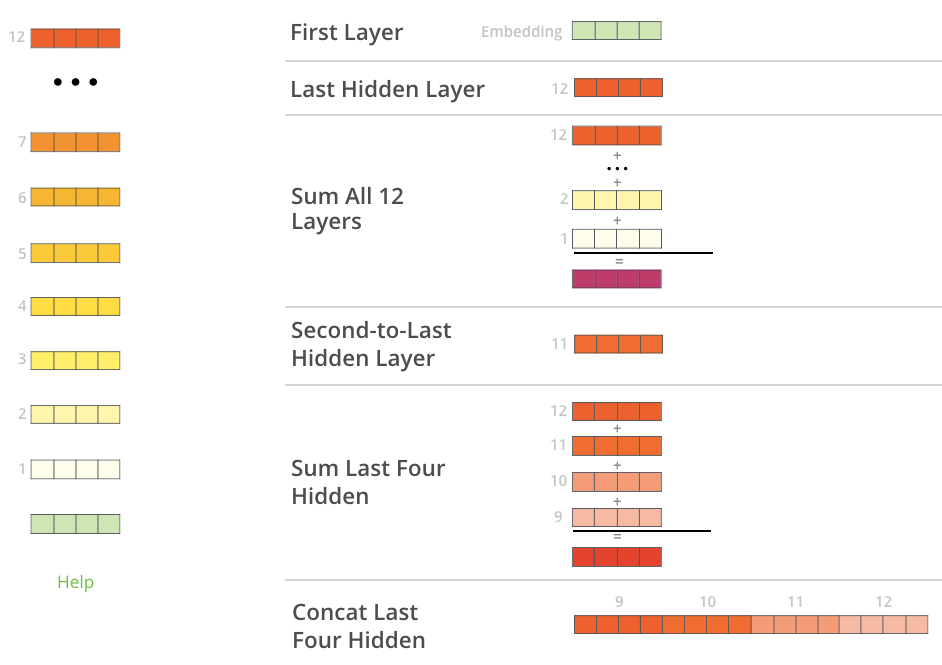
\includegraphics[width=11cm]{assets/pooling-strategy.png}
	\caption[Caption for LOF]{Pooling strategy. \cite{transformer}}
\end{figure}

\noindent
Nel caso in questione, si è scelto di concatenare gli ultimi 4 hidden layers e mediare tutti gli embeddings dei tokens presenti nel documento. In tutto si ottiene un vettore di 3072 elementi, il quale sarà utilizzato come features dei modelli in sostituzione della rappresentazione BOW \cite{berttutorial}.

\subsubsection{Sentence-BERT}
Sentence-BERT\cite{sentencebert} è una messa a punto della rete neurale BERT, permette di generare embeddings semanticamente validi relativi ad intere frasi.

\section{Caratteristiche linguistiche}
La scelta di features ad alto contenuto informativo ed indipendenti tra loro, è un passo fondamentale per un corretto riconoscimento di pattern nei dati.
A questo scopo vengono estratte delle caratteristiche linguistiche dal testo che sono rilevanti per il riconoscimento dell'ironia. Più le caratteristiche sono discriminanti quando si esprime un messaggio ironico, meglio si potranno distinguere le due classi. Queste features, insieme alla codifica testuale, verranno usate per creare il modello.

\subsection{PP (Pragmatic particles)}
Per catturare il senso non letterale racchiuso in ogni messaggio, vengono considerati alcuni elementi linguistici di seguito elencati.

\subsubsection{Emoticons}
Le emoticons sono riproduzioni stilizzate di quelle principali espressioni facciali umane che esprimono un'emozione. In accordo con l'assunzione che esista una relazione tra il sentimento espresso e l'ironia, queste vengono distinte in due categorie:
\begin{itemize}
	\item
	\textbf{Positive: } Es. ':-)', ':-D'
	\item
	\textbf{Negative: } Es. ':-(', ':=('
\end{itemize}
Viene quindi considerata l'occorrenza di emoticons positive e negative presenti in un tweet.

\subsubsection{Acronimi}
Gli acronimi sono un ulteriore strumento della comunicazione non verbale. Come le emoticons vengono presi in considerazione dal momento che possono esprire sentimenti positivi o negativi, infatti possiamo anch'essi dividerli in due categoire:

\begin{itemize}
	\item
	\textbf{Positivi}: Es. 'ROLF' (Rolling On Floor Laughing), 'LHO' (Laughing Head Off)
	\item
	\textbf{Negativi}: Es. 'BM' (Bad Manner)
\end{itemize}
Anche in questo caso si considera l'occorrenza di acronimi positivi e negativi.

\subsubsection{Espressioni onomatopeiche}
L'uso di espressioni onomatopeiche come 'boom' o 'clap' possono essere utilizzate nell'esprimere un messaggio ironico. Tuttavia in questo caso viene presa in considerazione solo la frequenza di queste espressioni, al contrario di come visto in precedenza per le emoticons e gli acronimi, dove si valutava anche la polarità.

\subsubsection{Punteggiatura}
La punteggiatura nei social media non segue le convenzioni ortografiche: Ad esempio 'Do you hear us now ?????'\\
Per questa ragione si considera la frequenza di:
\begin{itemize}
	\item \textbf{Virgole}
	
	\item \textbf{Punti di domanda}
	
	\item \textbf{Punti escalmativi}
\end{itemize}

\subsubsection{Estrazione particelle pragmatiche}
Di seguite viene mostrato un esempio di come le particelle pragmatiche vengono estratte da un messaggio:

\begin{lstlisting}[caption={Esempio di tweet processato per estrarre le particelle pragmatiche.}]
Tweet: ':D lmao! RT @KarlDetkenProDJ iPad Humor Steve, I'ma let you finish,
        but Moses had the greatest  tablet of all time ;) clap clap'
Emot (-, +)  >>> [0, 2]
Init (-, +)  >>> [0, 1]
Onom (#)     >>> [2]
Punct        >>> {',': 2, '!': 1, '?': 0}
\end{lstlisting}


\subsection{POS (Part Of Speech)}
La struttura delle frasi che costituiscono il tweet, può essere un indicatore per il riconoscimento dell'ironia. A questo scopo viene tenuta in considerazione la frequenza dei POS (part-of-speech) tags presenti in un messaggio.

Per associare i POS tag ad ogni tweet viene utilizzato il POS tagger Noah's ARK \cite{ark} specifico per il dominio considerato. Si procede con la tokenizzazione del tweet per poi associare ad ognuno di questi il corretto tag. Di seguito la lista di tags considerati:\\


\begin{varwidth}[t]{\textwidth}
	\textbf{Nominale}
	\begin{itemize}
		\item \textbf{N}: Nome comune
		\item \textbf{O}: Pronome personale
		\item \textbf{\^}: Nome proprio
		\item \textbf{S}: Nominale + Possessiva
		\item \textbf{Z}: Nome proprio + Possessiva
	\end{itemize}
\end{varwidth}
\hspace{4em}
\begin{varwidth}[t]{\textwidth}
	\textbf{Closed-class words}
	\begin{itemize}
		\item \textbf{D}: Determiner
		\item \textbf{P}: Pre/Post-posizione;\\Congiunzione subordinante
		\item \textbf{\&}: Congiunzione coordinante
		\item \textbf{T}: Verb particles
		\item \textbf{X}: Existential there
	\end{itemize}
\end{varwidth}\\\\

\begin{varwidth}[t]{\textwidth}
	\textbf{Open-class words}
	\begin{itemize}
		\item \textbf{V}: Verbo
		\item \textbf{A}: Aggettivo
		\item \textbf{R}: Avverbio
		\item \textbf{!}: Interiezioni
	\end{itemize}
\end{varwidth}
\hspace{11em}
\begin{varwidth}[t]{\textwidth}
	\textbf{Composti}
	\begin{itemize}
		\item \textbf{L}: Nominale + Verbo (e.g.: I'm)
		\item \textbf{M}: Nome proprio + Verbo
		\item \textbf{Y}: X + Verbo
	\end{itemize}
\end{varwidth}\\\\\\\\
Di seguito è mostrato un esempio di POS tags associati al tweet passando per i tokens:


\begin{lstlisting}[caption={Esempio di tweet con POS tags associati.}]

Tweet: 'Need a second opinion? Who gave you the first one?'
Tokens  >>> [Need], [a], [second], [opinion], [?], [Who],
            [gave], [you], [the], [first], [one], [?]
Tags    >>> ['V', 'D', 'A', 'N', ',', 'O', 'V', 'O', 'D', 'A', '$', ',']
Freq.   >>> {'N': 1, 'O': 2, '^': 0, 'S': 0, 'Z': 0, 'V': 2,
             'A': 2, 'R': 0, '!': 0, 'D': 2, 'P': 0, '&': 0,
             'T': 0, 'X': 0, 'L': 0, 'M': 0, 'Y': 0}
\end{lstlisting}
Come si può notare, il POS tagger associa dei tags che non sono stati elencati sopra, questi verranno semplicemente ignorati e non utilizzati come features per il modello. 

\subsection{EMOT (Emotional Features)}
Alcune teorie psicologiche suggeriscono l'esistenza di emozioni primarie. Su questo si basano i lessici EmoLex e EmoSenticNet, in cui vengono riportate le sfere emotive a cui appartengono le parole.
I lessici si possono intendere come diversi insiemi che caratterizzano le emozioni primarie, dove ognuno di questi insiemi è composto dalle parole che sono considerate appartenenti a quella specifica categoria emotiva. Si noti che insiemi considerati non devono necessariamente essere disgiunti.\\
Qualche esempio di seguito:

$birthday \in JOY \land birthday \in SURPRISE \land birthday \in ANTICIPATION$

$honor \in TRUST$

$ stair \notin (JOY \cup SURPRISE \cup ANTICIPATION \cup TRUST) $\\

Come feature aggiuntiva, dato un tweet tokenizzato si procede scorrendo le parole e consultando i diversi lessici. Per ogni parola presente nel tweet, si recuperano le sfere emotive a cui essa è associata. Una volta eseguita l'operazione per tutte le parole del tweet, si calcola la frequenza totale di ogni emozione.

I due lessici si basano su differenti teorie che identificano ognuna le proprie emozioni primarie, per questo motivo si combina il risultato di entrambe sommando le frequenze ottenute da ognuna delle due risorse.

\begin{table}[h!]
	\centering
	\begin{tabular}[t]{l|l}
		\hline
		\textbf{Emozione} & \textbf{Lessico} \\
		\hline
		Anger			& EmoLex, EmoSenticNet \\
		Anticipation	& EmoLex \\
		Disgust			& EmoLex, EmoSenticNet \\
		Fear			& EmoLex, EmoSenticNet \\
		Joy				& EmoLex, EmoSenticNet \\
		Sadness			& EmoLex, EmoSenticNet \\
		Suprise			& EmoLex, EmoSenticNet \\
		Trust			& EmoLex \\
		\hline
	\end{tabular}
	\caption{Emozioni primarie dei lessici.}
\end{table}

\noindent
Un esempio di come vengono estratte le features emozionali da un tweet:

\begin{lstlisting}[caption={Esempio di estrazione delle emozioni da un tweet.}]

Tweet: 'I nominate @MrsStephenFry for a Shorty Award in because... why
        not? http://bit.ly/shorty'
Words	     >>> ['nominate', 'shorty', 'award']
EmoLex       >>> {'anger': 0, 'anticipation': 1, 'disgust': 0, 'fear': 0,
                  'joy': 1, 'sadness': 0, 'surprise': 1, 'trust': 1}
EmoSenticNet >>> {'anger': 0, 'disgust': 0, 'joy': 3, 'sadness': 0,
                  'surprise': 0, 'fear': 0}
Combined     >>> {'sadness': 0, 'anticipation': 1, 'fear': 0, 'anger': 0,
                  'joy': 4, 'disgust': 0, 'trust': 1, 'surprise': 1}
\end{lstlisting}

\subsection{Sintesi features utilizzate}
Viene sotto riportata la tabella delle features utilizzate con il relativo numero:

Oltre alle caratteristiche linguistice, bisogna prendere in considerazione la rappresentazione del testo. Nel caso BOW dipende dalla cardinalità del dizionario. In questo caso, dagli esperimenti è emerso che, dopo l'opportuno filtraggio dei tokens \ref{section:filtering}, considerando tutto il dataset a disposizione il dizionario contiene 3967 tokens univoci.

Nel caso di BERT invece, le features dipendono dalla pooling strategy adottata. Dal momento che ognuno dei 12 hidden layers della rete neurale fornisce in output un vettore composto da 768 elementi, e negli esperimenti eseguiti si è scelto di concatenare gli ultimi 4 layers, nella rappresentazione del testo mediante BERT vengono considerate 3072 features.


\begin{table}[H]
	\centering
	\begin{tabular}[t]{l|c}
		\hline
		\textbf{Caratteristica} & \textbf{\#features} \\
		\hline
		Emoticons  			 & 2 \\
		Acronimi & 2 \\
		Espressioni onomatopeiche  & 1 \\
		Punteggiatura & 3 \\
		Part Of Speech & 17 \\
		Emotional features & 8 \\
		\hline
		& 33 \\
		
	\end{tabular}
	\caption{Features utilizzate.}
\end{table}


\chapter{Modelli supervisionati}
\label{chap:supervised-models}

Il machine learning è lo studio di algoritmi che migliorano automaticamente attraverso l'esperienza, ed è una branca dell'intelligenza artificiale. Il machine learning crea modelli matematici basati sui dati, i quali vengono utilizzati per far apprendere alla macchina, con lo scopo di fare previsioni o decidere riguardo dati che non sono mai stati visti prima.


\begin{figure}[H]
	\centering
	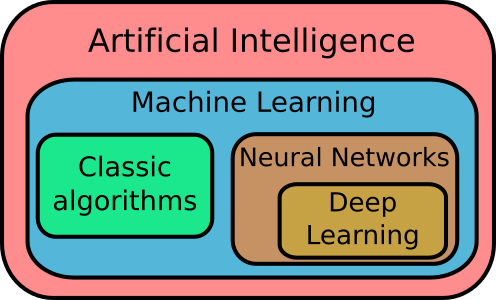
\includegraphics[width=7cm]{assets/ai_diagram.png}
	\caption[Caption for LOF]{Diagramma intelligenza artificiale.\footnotemark}
	\label{fig:artificial-intelligence}
\end{figure}

\footnotetext{Fonte: \url{http://medium.com/@vashkelis/machine-learning-in-5-minutes-9a6cce23ce7e}.}

In questa tesi vengono creati modelli supervisionati tramite l'utilizzo di algoritmi definiti "classici". Per apprendere dai dati ed estrarre dei pattern da questi, come input degli algoritmi, oltre al testo codificato e le features estratte, è necessario l'utilizzo delle relative etichette. Questa informazione aggiuntiva viene usata nella fase di apprendimento e indica a priori la relativa classe di appartenenza delle istanze che compongono il dataset. 

Esistono diversi algoritmi per creare modelli supervisionati, quelli utilizzati per gli esperimenti delle tesi sono:
\begin{itemize}
	\item Decision Tree
	\item Multinomial Naive Bayes
	\item Bayesian Network
	\item Support Vector Machine - Kernel lineare
\end{itemize}

\section{Decision Tree}
Un albero di decisione è un modello predittivo con una struttura ad albero. Ogni nodo interno rappresenta una feature, un arco verso un nodo figlio rappresenta un possibile valore per quella proprietà, ovvero una decisione, e una foglia il valore predetto. Il processo consiste in una sequenza di test, comincia sempre dal nodo radice, e procede verso il basso. A seconda dei valori rilevati in ciascun nodo, si otterrà un path che porterà ad un nodo foglia e quindi una classificazione.

\begin{figure}[!h]
	\centering
	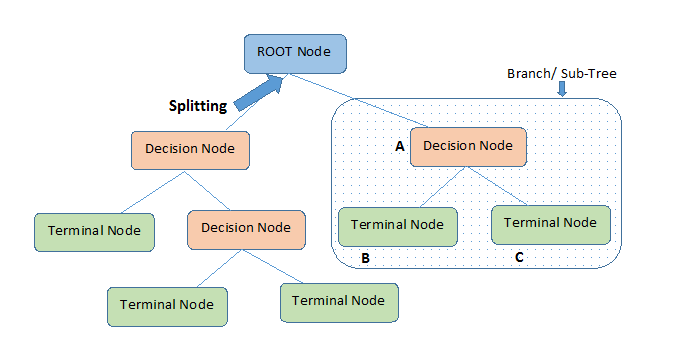
\includegraphics[width=13cm]{assets/decision_tree.png}
	\caption[Caption for LOF]{Albero di decisione.\footnotemark}
	\label{fig:decision-tree}
\end{figure}


\footnotetext{Fonte: \url{http://medium.com/datadriveninvestor/decision-tree-algorithm-with-hands-on-example-e6c2afb40d38}.}


Gli alberi di decisione hanno il vantaggio della semplicità. Infatti è possibile seguire il percorso radice-foglia per analizzare come la macchina è giunta a una determinata decisione basandosi sui dati in input. Questo processo rappresenta di fatto la logica utilizzata dalla macchina per interpretare i dati.

Un problema degli alberi di decisione è che tendono ad andare in overfitting.

\newpage
\section{Naive Bayes}
L'algoritmo di classificazione Naive Bayes si basa sull'applicazione del teorema di Bayes:
$$P(A \mid B) = \frac{P(B \mid A)P(A)}{P(B)}$$
Contestualizzato per la creazione di un modello per un task di classificazione, si ha la tupla composta dalle features di un particolare documento:

$$\textbf{x} = (x_1, ..., x_n)$$
Applicando il teorema di Bayes, rappresentando $y$ come la classe a cui appartiene un individuo, si ottiene:

$$P(y|\textbf{x}) =
\frac{P(\textbf{x}\ |\ y)P(y)}{P(\textbf{x})}$$
Si noti che la parte destra dell'uguaglianza è la probabilità a priori, ed è stimabile utilizzando il dataset a disposizione. In particolare il numeratore rappresenta la probabilità:

$$P(\textbf{x} \cap y) = P(x_1, ..., x_n, y)$$
Viene sviluppata la probabilità congiunta utilizzando la chain rule per l'applicazione ripetuta della porbabilità condizionata:




\begin{align}
\begin{split}\label{eq:1}
P(x_1, ..., x_n, y){} &=  P(x_1 \,|\, x_2, ..., x_n, y)P(x_2, ..., x_n, y)\\
&= P(x_1 \,|\, x_2, ..., x_n, y)P(x_2\, |\, x_3, ..., x_n, y)P(x_3, ..., x_n, y)\\
&= ...\\
&= P(x_1 \,|\, x_2, ..., x_n, y)P(x_2\, |\, x_3, ..., x_n, y)...P(x_{n-1}\,|\,x_n,y)P(x_n \mid y)P(y)\\
\end{split}
\end{align}
Il classificatore preso in questione è considerato "naive", in quanto si assume che le features siano indipendenti tra loro, pertanto:
$$P(x_i\,|\, x_{i+1}, ...,x_n, y) = P(x_i \mid y)$$
Si procede quindi sviluppando l'equazione per il calcolo della probabilità a posteriori:
$$P(y \mid x_1, x_2, ..., x_n) =
\frac
	{P(x_1 \mid y)...P(x_n \mid y)P(y)}
	{P(x_1)...P(x_n)}$$
A questo punto, date le features di un individuo, è possibile calcolare la probabilità che questo appartenga ad una particolare classe $y$. Inoltre, fissate le fetures, il denominatore è costante. Si considera quindi:
$$P(y \mid x_1, x_2, ..., x_n) \propto
P(y)\prod\limits_{i=1}^{n}P(x_i \mid y)
$$
Un individuo viene classificato come quella classe $y$ che massimizza la probabilità a posteriori:
$$\hat{y} = \argmax_y P(y)\prod\limits_{i=1}^{n}P(x_i \mid y)$$


\section{Multinomial Naive Bayes}
Nell'algoritmo Naive Bayes, avendo dati n-dimensionali e k classi, la probabilità a posteriori si ottiene conoscendo $P(x_i \mid y_j)$ per ogni $1\leq n,\ 1\leq j \leq k$

Queste probabilità vanno stimate dal dataset, e nella variante Multinomial Naive Bayes si considera una distribuzione binomiale in più variabili (da qui multinomiale). Si hanno quindi i parametri $\theta_y = (\theta_{y1}, \theta_{y2}, ...\theta_{yn})$, dove $\theta_{yi} = P(x_i \mid y)$ vengono stimati in questo modo:

$$\hat{\theta}_{yi} = \frac{N_{yi} + \alpha }{N_{y} + \alpha n}$$
Dove, indicando con $T$ il training set:
$$N_{yi} = \sum_{x \in T}x_i \qquad
N_{y} = \sum_{i=1}^{n}N_{yi}$$
Il parametro $\alpha: 0 < \alpha \leq 1$ è chiamato di smoothing, e ha lo scopo di gestire quei casi in cui una features non è presente nel training set, così da non ottenere probabilità uguali a $0$.

\section{Bayesian Network}
I classificatori naive Bayes si basano sull'assunzione di indipendenza delle caratteristiche. Ciò permette di semplificare le cose quando si considera l'equazione \eqref{eq:1} come risultato dell'applicazione della chain rule.
Tuttavia questa è un'assunzione piuttosto forte.

A questo scopo i classificatori Bayesian Network introducono una struttura dati per far fronte a questo problema. Viene pertanto considerato un DAG (Directed acyclic graph) in cui le $n$ features compongono i nodi del grafo, e gli archi rappresentano la dipendenza tra le variabili.

\begin{figure}[!h]
	\centering
	\begin{subfigure}[b]{0.4\textwidth}
		\centering
		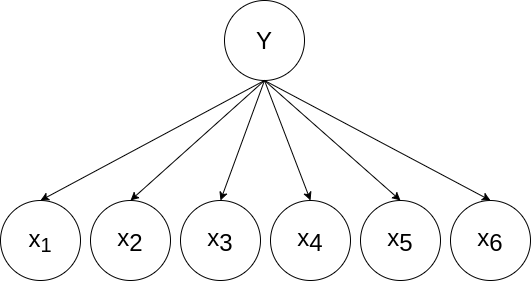
\includegraphics[width=\linewidth]{assets/naive-bayes.png}
		\caption{Naive Bayes network}
		\label{fig:naive-bayes}
	\end{subfigure}
	\hfill
	\begin{subfigure}[b]{0.4\textwidth}
	\centering
		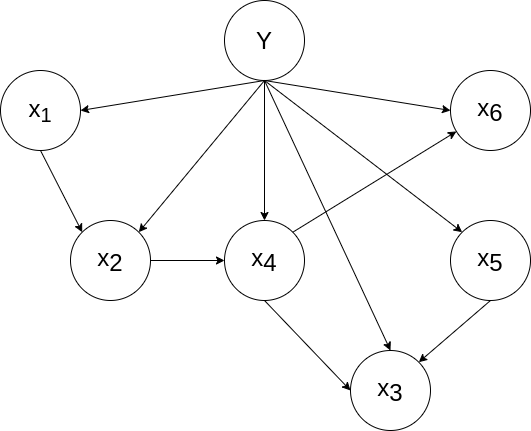
\includegraphics[width=\linewidth]{assets/bayes-network.png}
		\caption{Bayes network per problema specifico}
		\label{fig:naive-bayes}
	\end{subfigure}
	\caption{Dipendenza tra variabili.}
\end{figure}
\noindent Considerando le $n$ features indipendenti tra loro si ha:
$$P(X_1, ..., X_n) = \prod\limits_{i=1}^{n}P(X_i) $$
Senza questa assunzione si applica la chain rule per la probabilità congiunta, la quale è computazionalmente onerosa:

\[ 
P \left( \bigcap_{i=1}^n X_i \right) = 
\prod\limits_{i=1}^{n}P
\left( X_i  \bigg\vert
\bigcap_{j=1}^{i-1} X_j \right)
\]
Tuttavia si sfrutta il grafo diretto aciclico G così definito:
\begin{itemize}
	\item $G = (V, E)$
	\item $V = \{X_1, ..., X_n\}$
	\item $E = \{(U,V) \mid (U,V) \in V^2 \land P(U, V) = P(V \mid U)P(U) = P(U \mid V)P(V) \}$
\end{itemize}
Il quale rappresenta le dipendenze tra variabili. Quindi nello sviluppo della probabilità congiunta, si considerano solo quei fattori con un arco presente nel grafo. Pertanto, indicando con $\pi(u) = \{v \mid (v, u) \in E\}, v,u \in V$ si ha:


$$P(X_1, ..., X_n) = \prod\limits_{i=1}^{n}P(X_i \mid X_{i+1}, ..., X_{n}) = \prod\limits_{i=1}^{n}P(X_i \mid \pi(X_i)) $$
Così facendo viene semplificata la probabilità congiunta, pur non assumendo la mutua indipendenza tra le variabili.

\newpage
\section{Support Vector Machine}
Support vector machine è un'altro algoritmo di machine learning supervisionato, in cui gli $n$ individui sono rappresentati nella forma:
$$(\vec{x}_1, y_1),...,(\vec{x}_n, y_n)$$
Dove $y_i \in \{1, -1\}$ rappresenta la classe di appartenenza di un individuo. Ogni $\vec{x}_i$ è un vettore reale k-dimensionale, con tante dimensioni quante sono le features.

\subsection{Iperpiano}
L'obbiettivo dell'algoritmo è trovare l'iperpiano ottimo che che meglio separa le due classi.
Nel caso 2-dimensionale, l'iperpiano è individuato da una retta, tuttavia è facilmente generalizzare il concetto al caso 3-dimensionale e così via:
\begin{figure}[H]
	\centering
	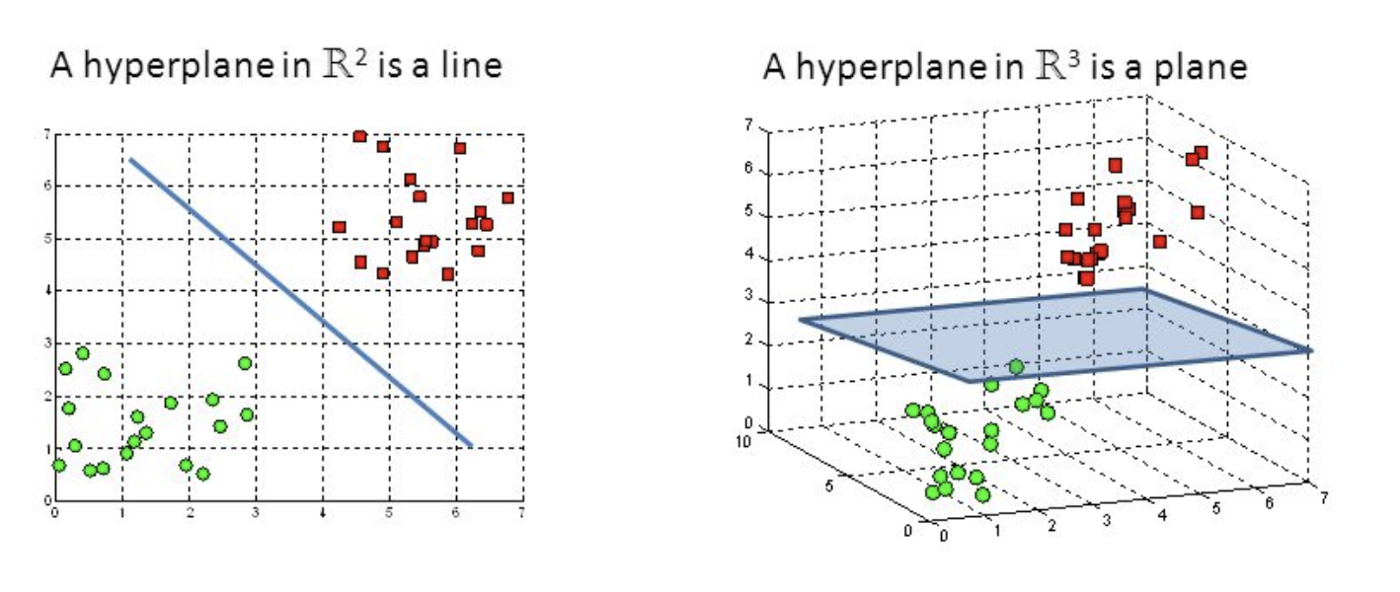
\includegraphics[width=12cm]{assets/svm-hyperplane.png}
	\caption[Caption for LOF]{Iperpiano ottimo.\footnotemark}
	\label{fig:svm-2d}
\end{figure}


\footnotetext{Fonte: \url{www.towardsdatascience.com/a-friendly-introduction-to-support-vector-machines-svm-925b68c5a079}.}


\subsection{Iperpiano ottimo}
Per iperpriano ottimo si intende quello che massimizza la distanza tra l'iperpiano e il più vicino punto $\vec{x}_i$ di ciascuna classe. Indicando con $\vec{w}$ il vettore normale all'iperpiano, ogni iperpiano può essere scritto come l'insieme dei punti $\vec{x}$ che soddisfano l'equazione:
$$\vec{w}\cdot\vec{x} - b = 0$$
Vengono considerati i due iperpiani paralleli che separano le due classi, la quale distanza tra i due è la più grande possibile. La regione compresa tra questi è detta margine, e l'iperpiano ottimo si trova nel mezzo tra i due. I due iperpiani possono essere scritti come:
$$\vec{w}\cdot\vec{x} - b = 1$$
$$\vec{w}\cdot\vec{x} - b = - 1$$
Essendo $\vec{w}$ il vettore normale all'iperpiano, la distanza tra i due è $\frac{2}{||\vec{w}||}$, pertanto per massimizzare la distanza si vuole minimizzare $ ||\vec{w}||$.

Si considerano inoltre i vincoli per esprimere che ogni punto deve cadere nel lato corretto rispetto al margine:
$$\vec{w}\cdot\vec{x} - b \geq 1,\ se\ y_i = 1$$
$$\vec{w}\cdot\vec{x} - b \leq - 1,\ se\ y_i = -1$$


\begin{figure}[h!]
	\centering
	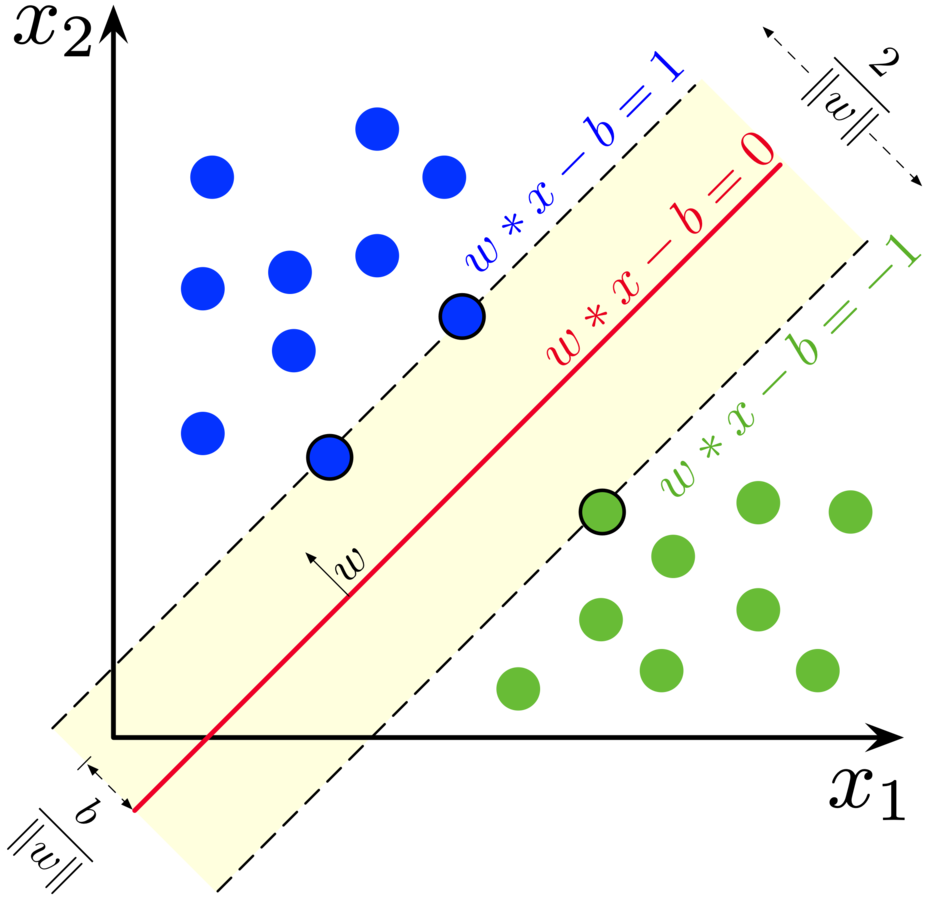
\includegraphics[width=7cm]{assets/svm-margin.png}
	\caption[Caption for LOF]{Margine SVM.\footnotemark}
	\label{fig:svm-margin}
\end{figure}

\footnotetext{Fonte: \url{www.wikipedia.org/wiki/File:SVM_margin.png}.}


\subsection{Vettori di supporto}
I due iperpiani che individuano il margine, sono trovati a partire dai vettori che appartengono al dataset. Quei punti che permettono di individuare le frontiere del margine, ovvero i due iperpiani paralleli, sono i vettori di supporto. Questi punti del dataset sono fondamentali, in quanto per costruzione cadono sul bordo del margine, pertanto lo spostamento o la rimozione di uno di essi, avrebbe come risultato due iperpiani diversi che definiscono il margine, quindi un differente iperpiano ottimo.

\subsection{SVM non lineare}
Fino ad ora sono stati presi in considerazione solo dataset linearmente separabili. Tuttavia questo può non essere sempre possibile. L'idea è quindi di mappare i dati in uno spazio con una dimensione in più, con lo scopo di ottenere la separazione lineare utilizzando un iperpiano nello spazio con una dimensione aggiuntiva.

Sotto viene preso come esempio un dataset in $R^2$ non separabile utilizzando un iperpiano. Si considerano quindi la trasformazione:


$$\phi \colon R^2 \to R^3$$
$$\phi(\boldsymbol{X})  = [x_1, x_2, x_1^2 + x_2^2]^T$$ 
Utilizzando tale trasformazione, il dataset di partenza viene mappato in uno spazio con una dimensione in più:


\begin{figure}[!h]
	\begin{subfigure}[b]{0.5\textwidth}
		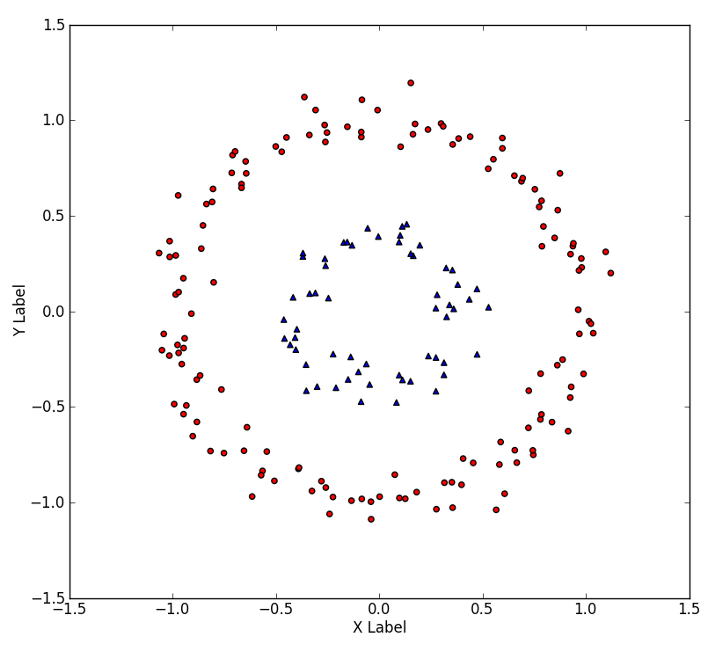
\includegraphics[width=\linewidth]{assets/svm-non-separable-1.png}
		\caption{Dataset in $R^2$}
		\label{fig:dataset-r2}
	\end{subfigure}
	\hfill
	\begin{subfigure}[b]{0.5\textwidth}
		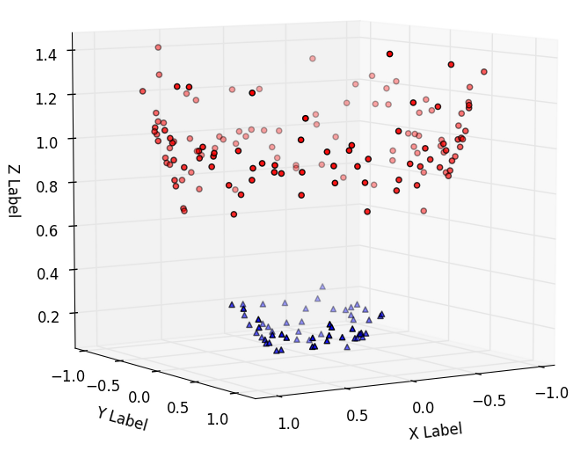
\includegraphics[width=\linewidth]{assets/svm-non-separable-2.png}
		\caption{Dataset trasformato in $R^3$}
		\label{fig:dataset-r3}
	\end{subfigure}%
	\caption[Caption for LOF]{Aggiunta di una nuova dimensione.\footnotemark}
\end{figure}

\footnotetext{Fonte: \url{www.medium.com/@vivek.yadav/why-is-gradient-descent-robust-to-non-linearly-separable-data-a50c543e8f4a}.}
\noindent
Dopo la trasformazione, come si può notare dalla figura~\ref{fig:dataset-r3}, è possibile trovare un iperpiano in $R^3$ che ben separa le due classi:

\begin{figure}[!h]

	\begin{subfigure}[b]{0.5\textwidth}
		
		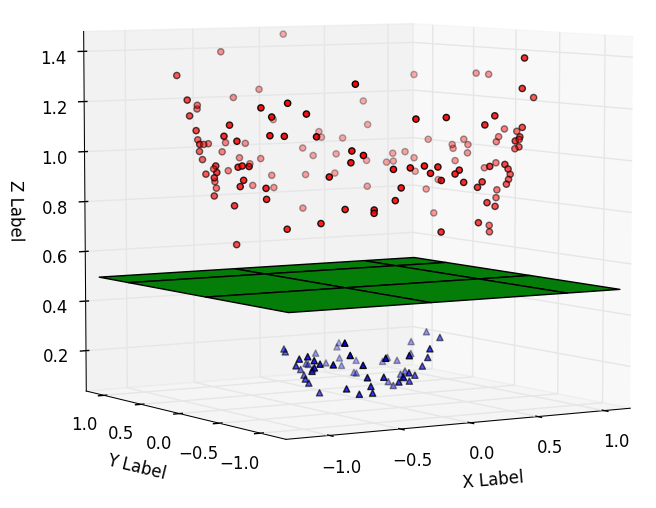
\includegraphics[width=\linewidth]{assets/svm-separable-1.png}
		\caption{Iperpiano in $R^3$}
		\label{fig:iperpiano-r3}
	\end{subfigure}
	\hfill
	\begin{subfigure}[b]{0.5\textwidth}
		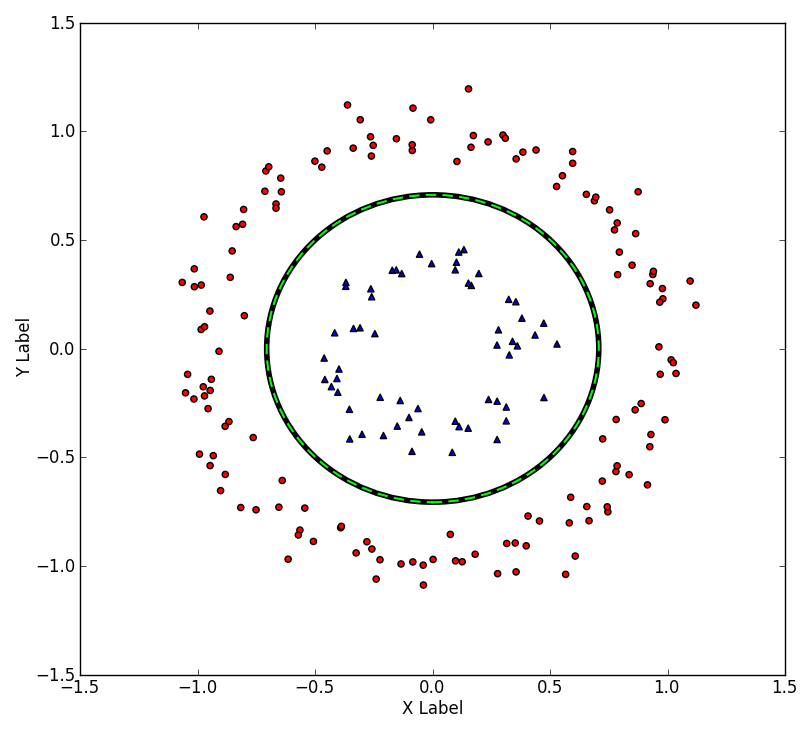
\includegraphics[width=\linewidth]{assets/svm-separable-2.png}
		\caption{Iperpiano proiettato in $R^2$}
		\label{fig:iperpiano-r2}
	\end{subfigure}%
	\caption[Caption for LOF]{Aggiunta di una nuova dimensione.\footnotemark}
\end{figure}

\footnotetext{Fonte: \url{https://www.eric-kim.net/eric-kim-net/posts/1/imgs/data_2d_to_3d_hyperplane.png}.}
\noindent
Nella figura~\ref{fig:iperpiano-r2}, è riportata la linea di dicisione per le due classi, ovvero l'iperpiano trovato in $R^3$ e poi proiettato in $R^2$.

\section{Strumenti utilizzati}
Per l'implementazione degli algoritmi, sono stati utilizzati degli strumenti che mettono a disposizione la possibilità di effettuare il training dei modelli.

\subsection{Scikit-learn}
Scikit-learn\cite{scikit-learn} è un modulo di python open soruce per il machine learning. Utilizzando questo modulo, è stato scritto il codice python per creare i modelli con gli algoritmi:
\begin{itemize}
	\item Decision Tree
	\item Multinomial Naive Bayes
	\item Support Vector Machine - Kernel lineare
	
\end{itemize}
Inoltre per ogni algoritmo sono stati creati più modelli considerando l'insieme potenza delle features. Quindi sono stati eseguiti i seguenti macrostep:
\begin{enumerate}
	\item Lettura del dataset
	\item Shuffle del dataset con lo stesso seed per ogni modello
	\item Standardizzare del dataset
	\item Creazione di 10 folds in cui viene effettuato lo split del dataset tra training-set e test-set
	\item Training dei modelli per ogni folds
	\item Valutazione dei classificatori per ogni folds
	\item Media delle misure di performance rispetto ogni folds
	\item Dump del report così da poter essere sucessivamente messo a confronto con altri modelli
\end{enumerate}
Essendo scikit-learn un modulo per python, che mette a disposizione delle API, è stato possibile gestire manualmente la politica per il training.

Infatti per questioni di ottimizzazione, fissato un algoritmo e con le relative features, è stato scelto di creare $k$ processi eseguiti in parallelo, ognuno dei quali si prende carico il training del modello su un particolare fold dei $k$ considerati. Avendo scelto per gli esperimenti 10 folds, ed utilizzato una macchina con 8 cores, ciò si presta bene per sfruttare ognuno degli 8 cores, con il risultato di ridurre il tempo totale impiegato per il training dei diversi modelli.

\subsection{Weka}

Weka\cite{weka} è un software open source per il machine learning. Questo applicativo può essere utilizzato attraverso interfaccia grafica, ed è in generale più immediato rispetto a scrivere del codice in python che utilizza le API fornite dal modulo scikit-learn. Con questo software sono stati creati i modelli utilizzando l'algoritmo:
\begin{itemize}
	\item Bayesian network
\end{itemize}
Non è stato utilizzato scikit-learn in quanto questo algoritmo non è implementato nel modulo.ttati tutti i cores per il training dei modelli.

\chapter{Campagna sperimentale}

\section{Dataset}
Il dataset a disposizione è il corpora \emph{TwReyes2013}, composto da 40,000 tweets in lingua inglese. Trattandosi di un approccio supervisionato, è richiesto che il dataset sia etichettato. Per associare una specifica label ai messaggi generati dagli utenti si possono seguire due strade:

\begin{itemize}
	\item \textbf{Self-Tagging}:
	\label{chap:self-taggin}
	Twitter mette a disposizione l'utilizzo degli hashtag nei messaggi. Assumendo che un utente utilizzi l'hashtag \emph{\#irony} con la volontà di esprimere ironia, è facile collezionare una serie di tweet etichettati come ironici.
	
	\item \textbf{Crowdsourcing}:	
	I vari tweet vengono etichettati manualmente da alcune persone
\end{itemize}
Per questo dataset la tecnica utilizzata è self-tagging considerando 4 hashtag diversi:


\begin{table}[ht]
	\centering
	\begin{tabular}[t]{llr}
		\hline
		\textbf{Numero} & \textbf{Hashtag}  & \textbf{Label assocaita}\\
		\hline
		10,000 & \emph{\#irony}     & ironico     \\
		10,000 & \emph{\#education} & non ironico \\
		10,000 & \emph{\#humor}     & non ironico \\
		10,000 & \emph{\#politics}  & non ironico \\
		\hline
	\end{tabular}
	\caption{Hashtag e label associate}
\end{table}%

\section{10-Folds Cross-Validation}
Per la fase di training dei modelli è necessario suddividere il dataset a disposizione in due diversi insiemi: training-set e test-set. Questo è un passaggio fondamentale in quanto non si otterrebbero delle misure di performance valide testando i modelli su dati che sono stati utilizzati per la fase di trainig. In pratica si vuole testare il modello su dati che non sono mai stati visti in precedenza.

Prima di iniziare la fase di training, i dati in input, che sono composti dalla matrice contenente le features estratte, vengono opportunamente mescolati. Con questo si intende che le righe della matrice vengono casualmente cambiate di posto, chiaramente mantenendo coerenza con le labels associate. Un aspetto importante è che lo shuffle della matrice è eseguito con lo stesso seed per tutti i modelli, così da ottenere delle misure di performance statisticamente valide.

Le performance ottenute, dipendono anche da come è stato diviso il dataset tra training-set e test-set. Per questo motivo viene utilizzata la tecnica k-Folds Cross-Validitation, che permette di sfruttare diverse porzioni di dati per i due insiemi. Il vantaggio di questa tecnica è quello di ottenere valutazioni più affidabile mediando i risultati di ognuno dei k modelli di cui è stato fatto il training, a discapito del tempo necessario, in quanto si effettuerà k volte il training di un modello.

Per gli esperimenti effettuati, è stato scelto $k=10$, ovvero il dataset è stato diviso 10 volte, utilizzando ad ogni iterazioni una porzione di dati diversa per il trainig-set e test-set. Avendo scelto questo valore di $k$, la proporzione tra i due insiemi sarà sempre $90\%$ per il training-set e $10\%$ per il test-set.

Nel seguente diagramma i pallini verdi e rossi individuano i tweets ironici e non ironici. Fissata un'istanza del dataset mescolato, si considera una sliding window di dimensione $\#samples \cdot \frac{1}{k}$, dove per ogni $k$ iterazione viene effettuato il training di un nuovo modello.

\begin{figure}[!h]
	\centering
	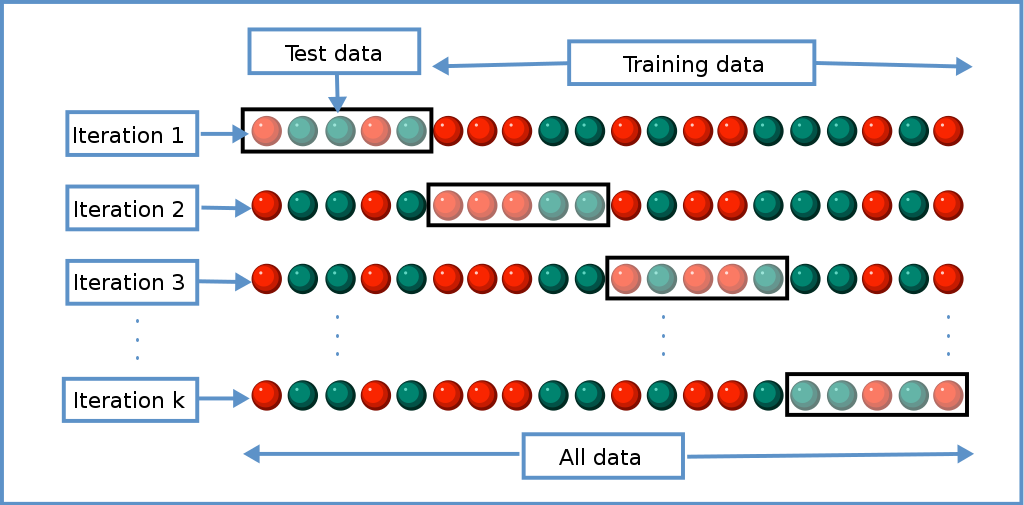
\includegraphics[width=13cm]{assets/cross-validation.png}
	\caption[Caption for LOF]{k-Folds Cross-Validation.\footnotemark}
	\label{fig:cross-validation}
\end{figure}


\footnotetext{Fonte: \url{www.wikipedia.org/wiki/Cross-validation_(statistics)}.}


\section{Misure di performance}
Essendo stati creati diversi modelli, è necessario valutarli. Avendo diviso il dataset a disposizione tra test-set e training-set, una volta completata la fase di training è possibile utilizzare il test-set per la valutazione. Si procede prendendo un tweet e facendolo classificare al modello, il quale verrà quindi identificato come ironico o non ironico. Trattandosi di modelli supervisionati, oltre ai dati si hanno a disposizione le labels associate, è quindi possibile confrontare l'output fornito dal modello con la reale classe di un tweet. Da qui si può capire se per quel particolare individuo la classificazione è corretta o meno.

Per la valutazione si utilizza tutto il test-set a disposizione e viene contano il numero di:
\begin{itemize}
	\item \textbf{TP} (True positive): Un tweet ironico è classificato come ironico - \emph{corretto}
	
	\item \textbf{TN} (True negative): Un tweet non ironico è classificato come non ironico - \emph{corretto}
	
	\item \textbf{FP} (False positive):	Un tweet non ironico è classificato come ironico - \emph{errato}
	
	\item \textbf{FN} (False negative):	Un tweet ironico è classificato come non ironico - \emph{errato}
\end{itemize}
Si noti che un modello può sbagliare la classificazione in due modi diversi, e c'è differenza tra classificare un tweet ironico come non ironico piuttosto che uno non ironico come ironico. Questi valori verranno poi analizzati sfruttando una matrice di confusione:

\begin{figure}[!h]
	\centering
	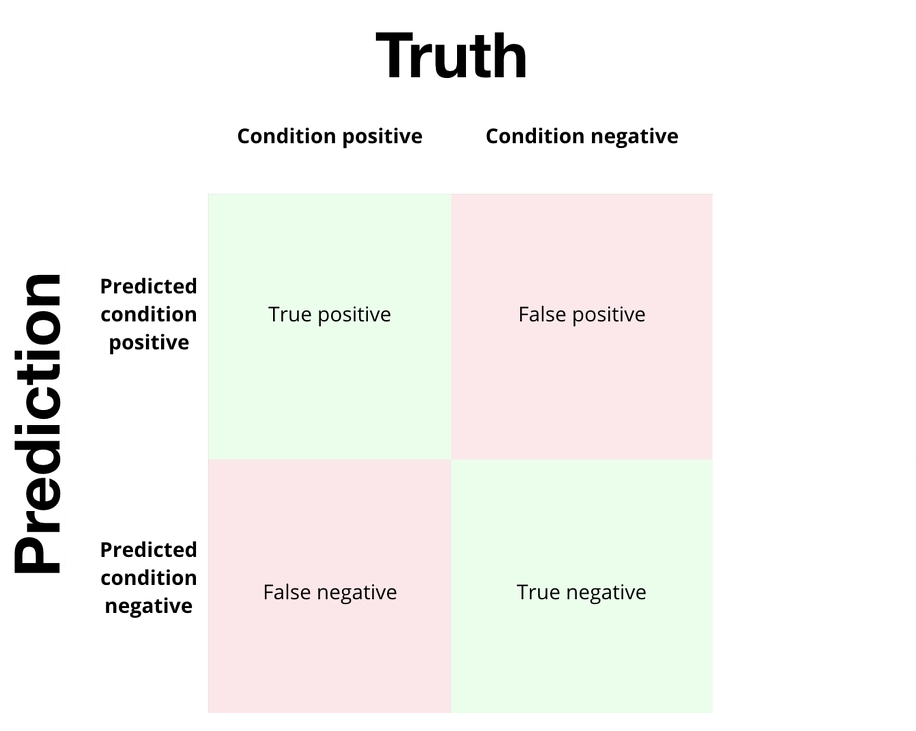
\includegraphics[width=10cm]{assets/confusion-matrix.jpg}
	\caption[Caption for LOF]{Confusion matrix.\footnotemark}
\end{figure}

\footnotetext{Fonte: \url{www.radiopaedia.org/cases/confusion-matrix-3}.}

Basandosi su questi dati vengono definite delle misure di performance per la valutazione:

\begin{itemize}
	\item \textbf{Accuracy}: Il rapporto tra il numero di classificazioni corrette e le classificazioni totali.
	
	$$Accuracy = \frac{TP + TN}{TP + FP + TN + FN} $$
	
	\item \textbf{Precision}: La porizione di classificazioni positive corrette.
	
	$$Precision = \frac{TP}{TP + FP} $$
		
	\item \textbf{Recall}: La porzione di sample positivi identificati.
	$$Recall = \frac{TP}{TP + FN} $$
	
	
	\item \textbf{F-measure}: Metrica per calcolare la valutazione complessiva. Formalmente è definita come la media armonica tra recall e precision.
	$$F\text{-}measure =  2 \cdot \frac{Precision \cdot Recall}{Precision + Recall} $$
	
\end{itemize}

\section{Esperimenti}
Avendo creato diversi modelli, questi sono stati confrontati per valutare il più performante. Nello specifico sono stati creati i modelli con gli algoritmi di classificazione:
\begin{itemize}
	\item Decision Tree
	\item Multinomial Naive Bayes
	\item Bayesian Network
	\item Support Vector Machine - Kernel lineare
\end{itemize}
Inoltre sia $F = \{text,\ pp,\ pos,\ emot\}$ l'insieme delle features considerate. Per ogni algoritmo di classificazione, sono stati creati i modelli utilizzando come features $\mathscr{P}(F)$.

\newpage
\subsection{Caratteristiche linguistiche}

\subsubsection{Weighted average}
\vfill
\begin{figure}[!h]
	\hspace*{-3cm}
	\begin{subfigure}[b]{0.5\textwidth}
		\centering
		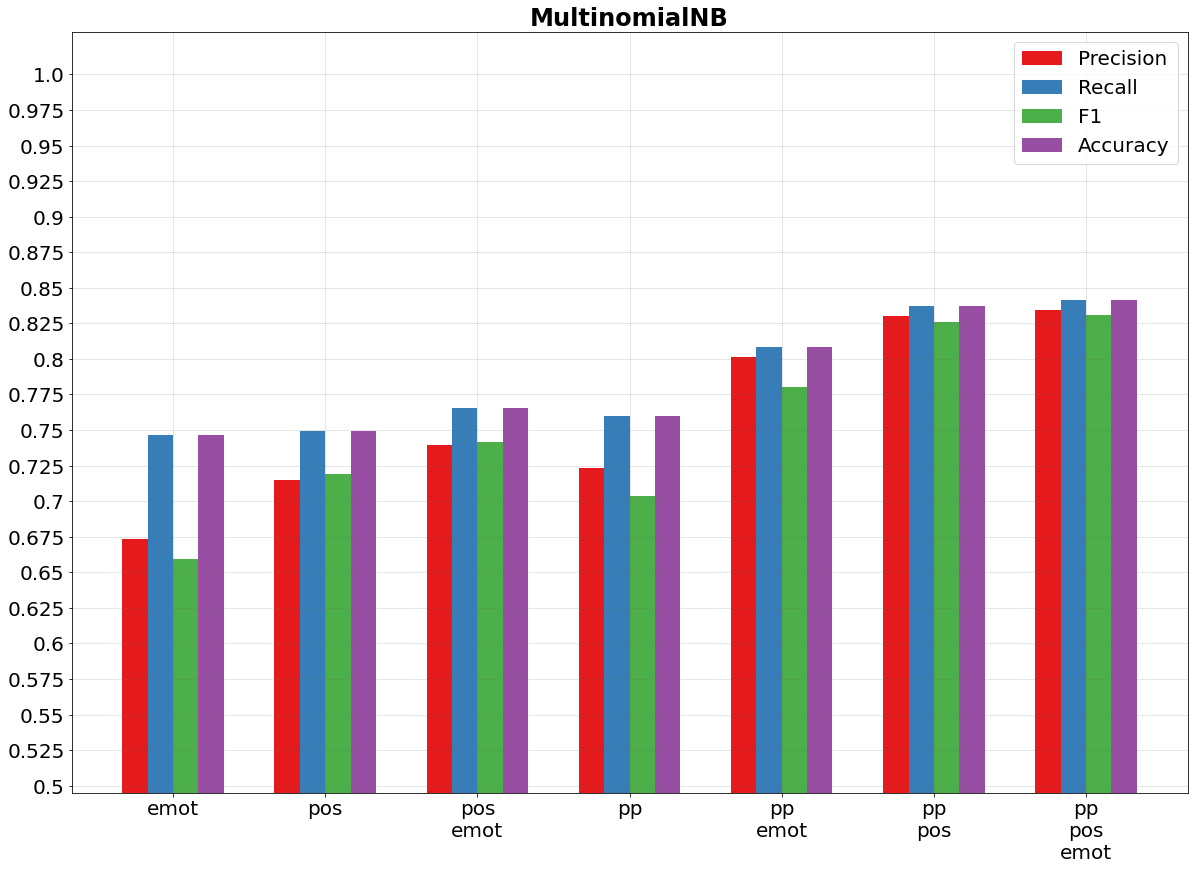
\includegraphics[width=10cm]{assets/reports/macro/nobow/MultinomialNB.png}
	\end{subfigure}
	\hfill
	\begin{subfigure}[b]{0.5\textwidth}
		\centering
		\hspace*{0.15cm}
		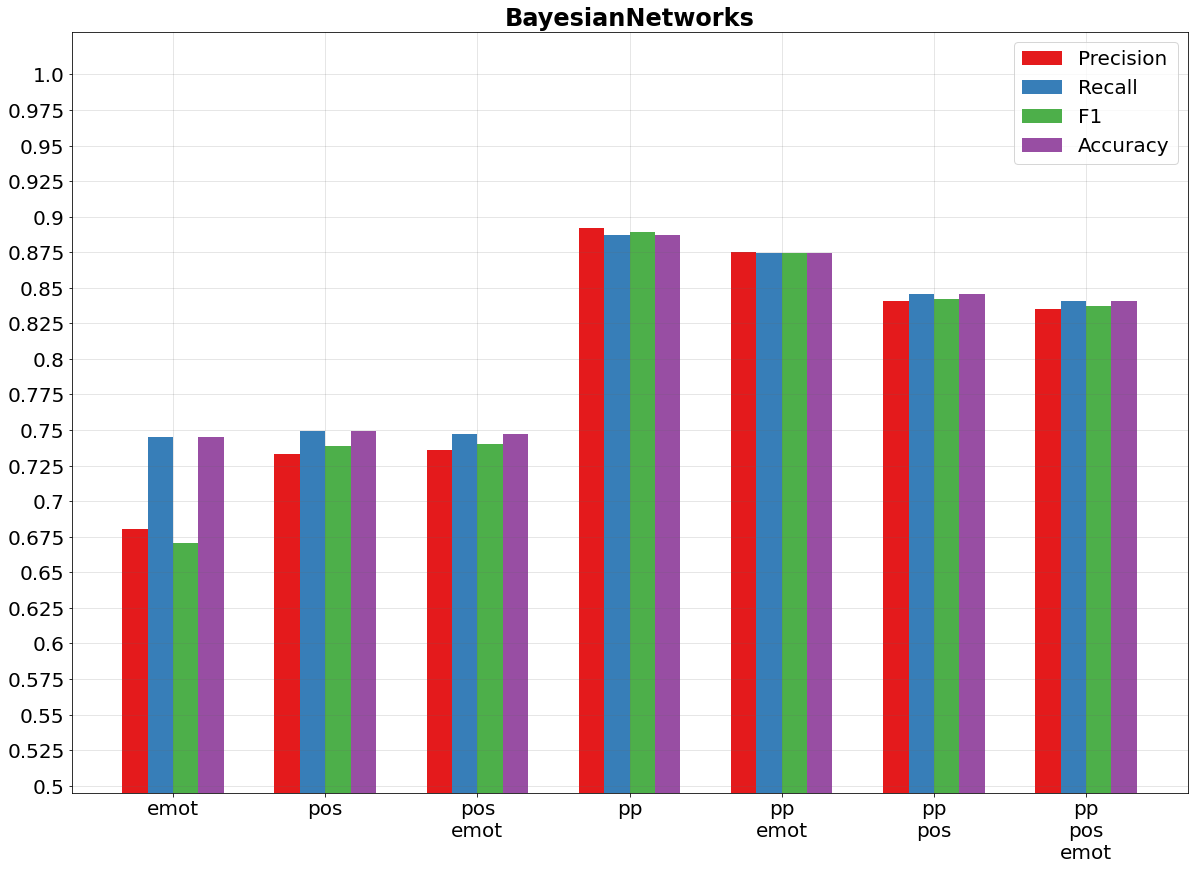
\includegraphics[width=10cm]{assets/reports/macro/nobow/BayesianNetworks.png}
	\end{subfigure}
\end{figure}
\vfill
\begin{figure}[!h]
	\hspace*{-3cm}
	\begin{subfigure}[b]{0.5\textwidth}
		\centering
		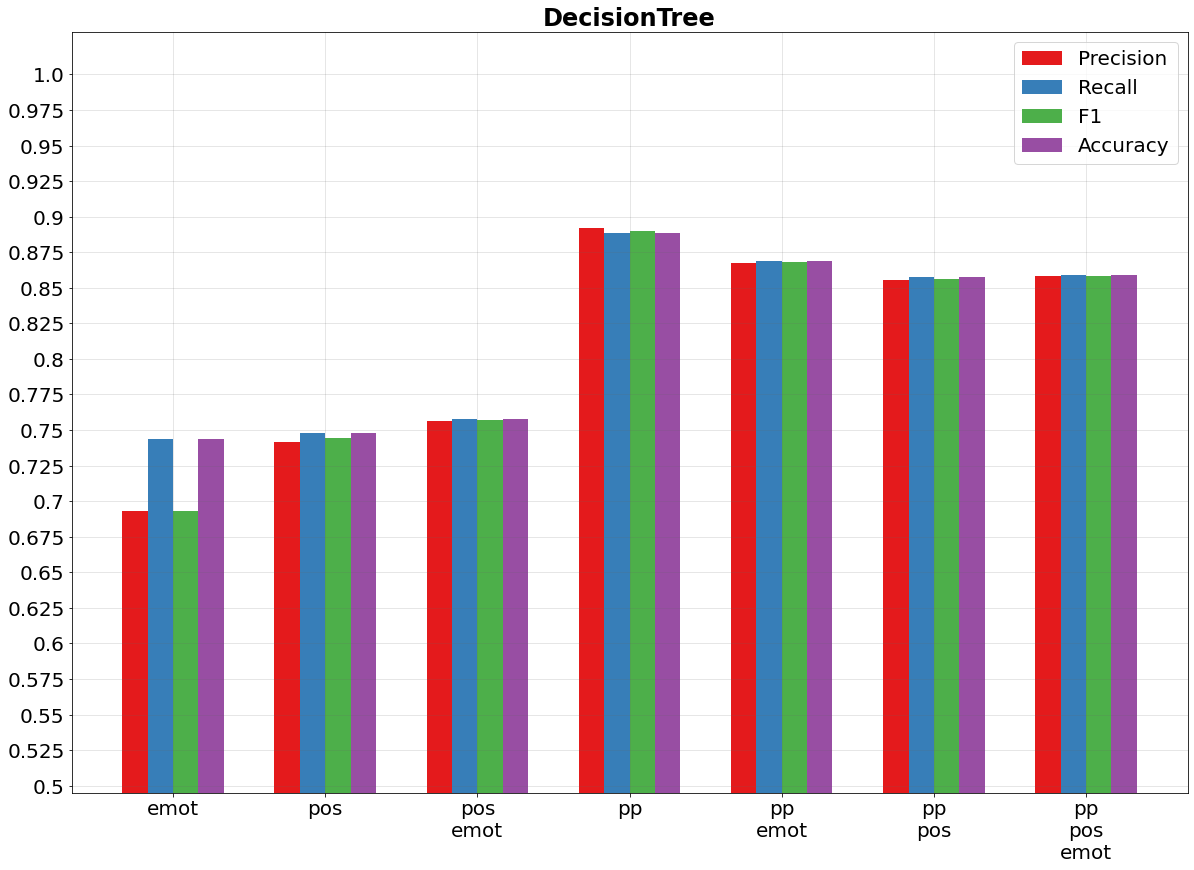
\includegraphics[width=10cm]{assets/reports/macro/nobow/DecisionTree.png}
	\end{subfigure}
	\hfill
	\begin{subfigure}[b]{0.5\textwidth}		
		\centering
		\hspace*{0.15cm}
		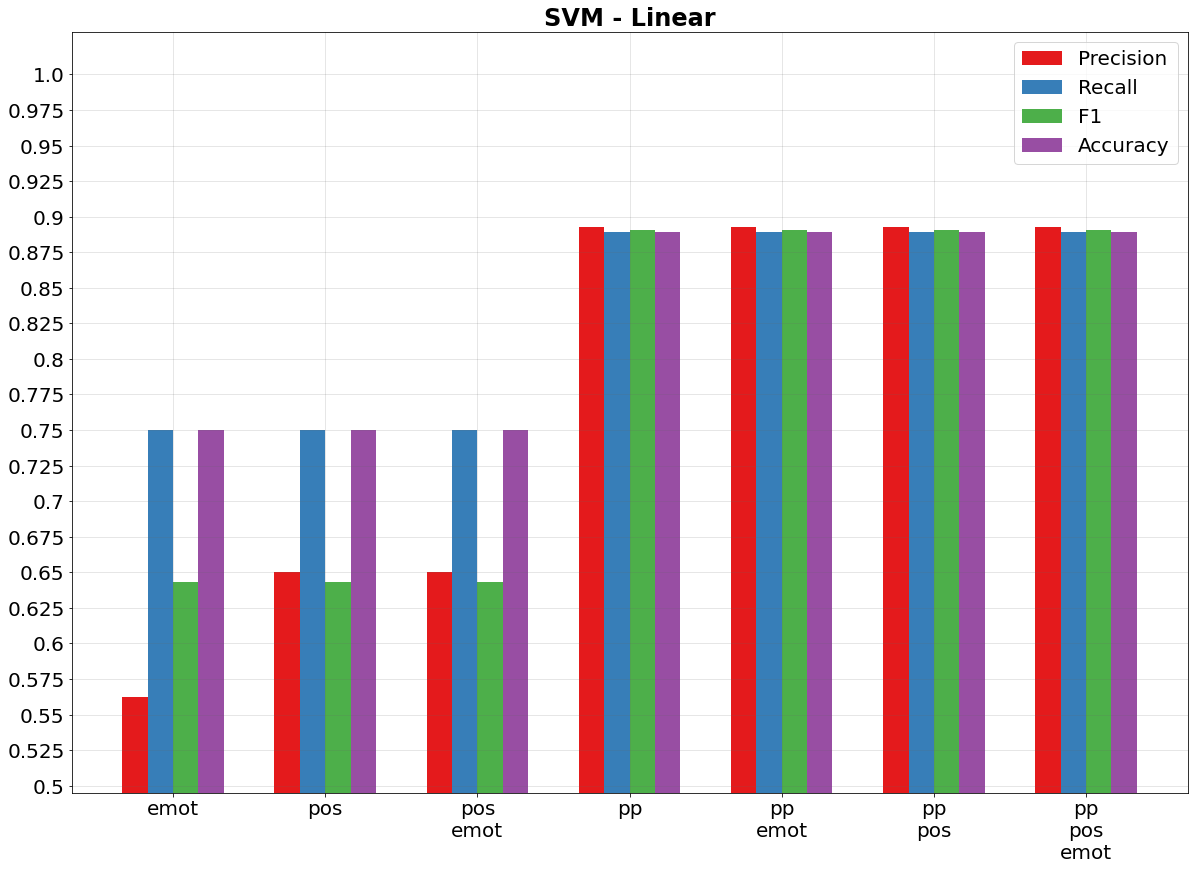
\includegraphics[width=10cm]{assets/reports/macro/nobow/SVM - Linear.png}
	\end{subfigure}
\end{figure}
\newpage

\begin{figure}[!h]
	\hspace*{-3cm}
	\begin{subfigure}[b]{0.5\textwidth}
		\centering
		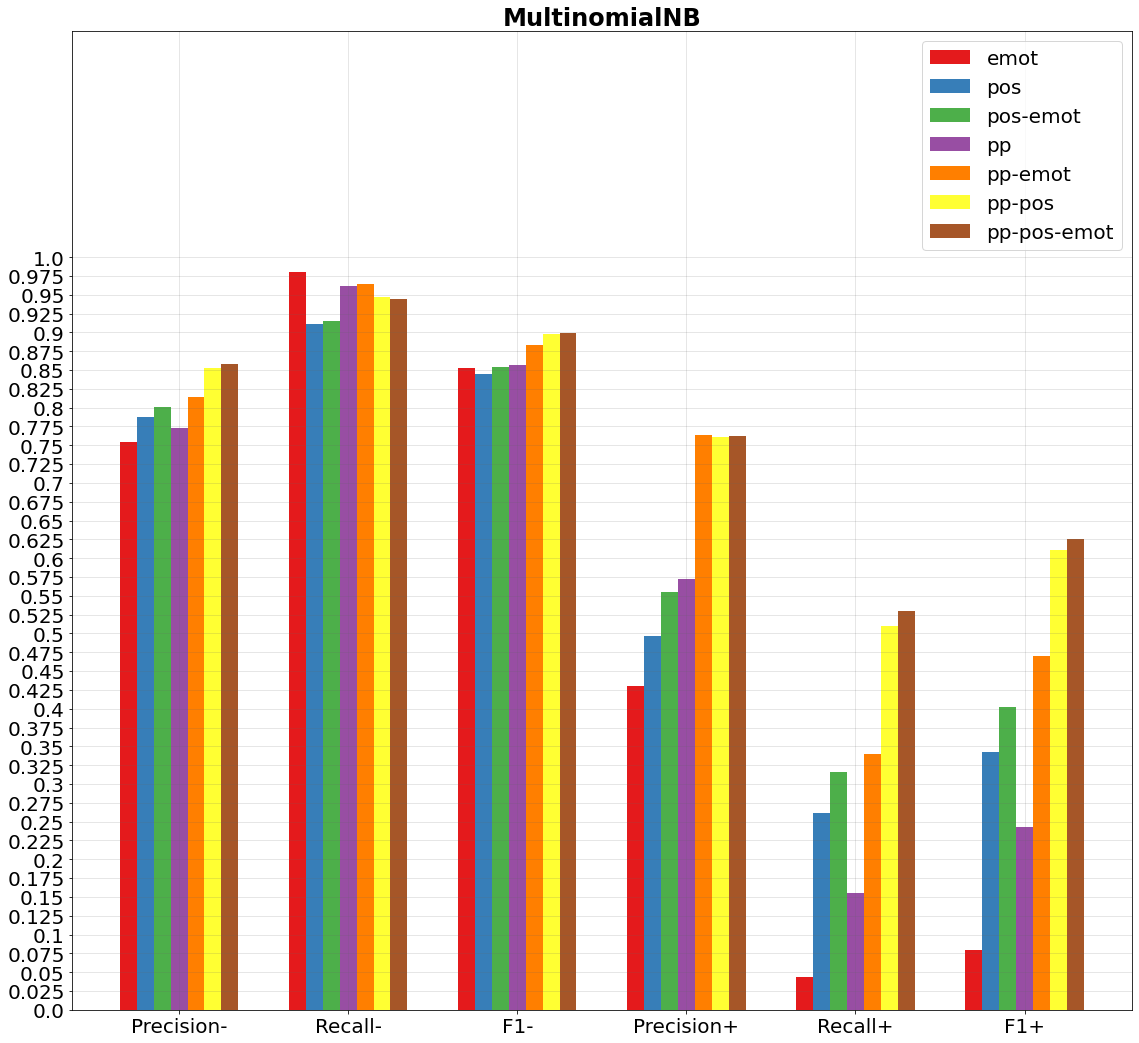
\includegraphics[width=10cm]{assets/reports/micro/nobow/MultinomialNB.png}
	\end{subfigure}
	\hfill
	\begin{subfigure}[b]{0.5\textwidth}
		\hspace*{0.15cm}
		\centering
		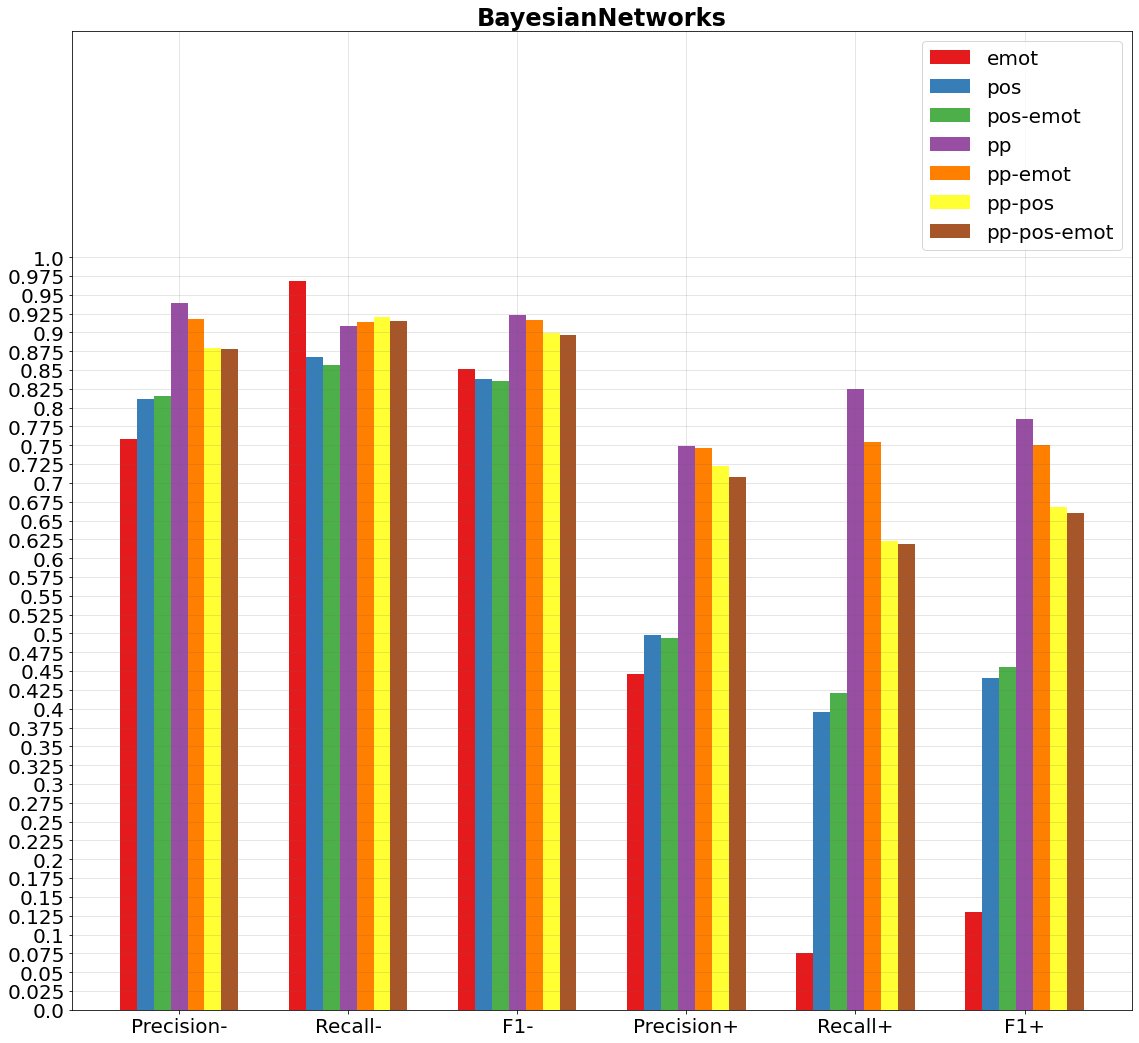
\includegraphics[width=10cm]{assets/reports/micro/nobow/BayesianNetworks.png}
	\end{subfigure}
\end{figure}
\vfill
\begin{figure}[!h]
	\hspace*{-3cm}
	\begin{subfigure}[b]{0.5\textwidth}
		\centering
		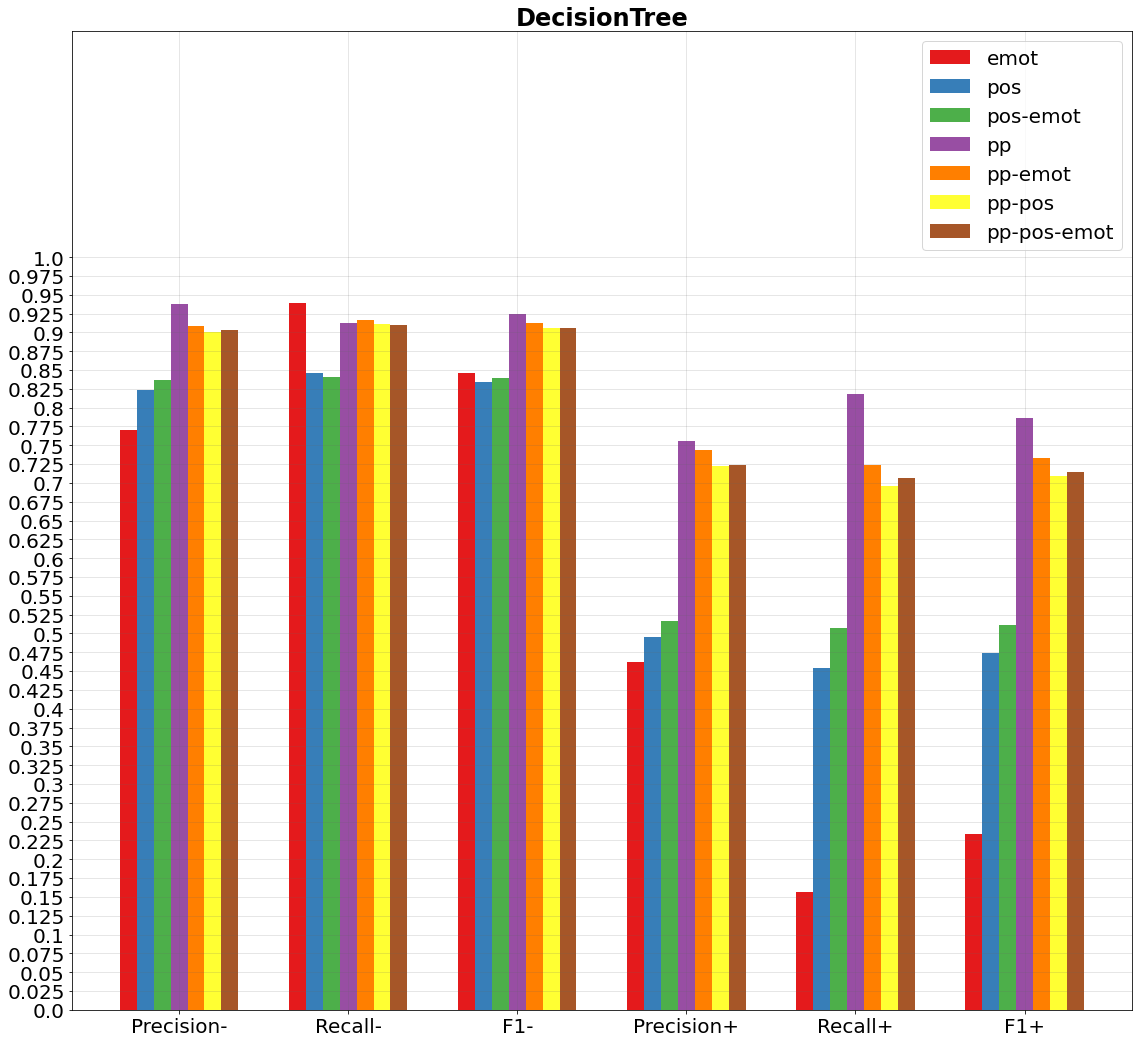
\includegraphics[width=10cm]{assets/reports/micro/nobow/DecisionTree.png}
	\end{subfigure}
	\hfill
	\begin{subfigure}[b]{0.5\textwidth}
		\centering
		\hspace*{0.15cm}
		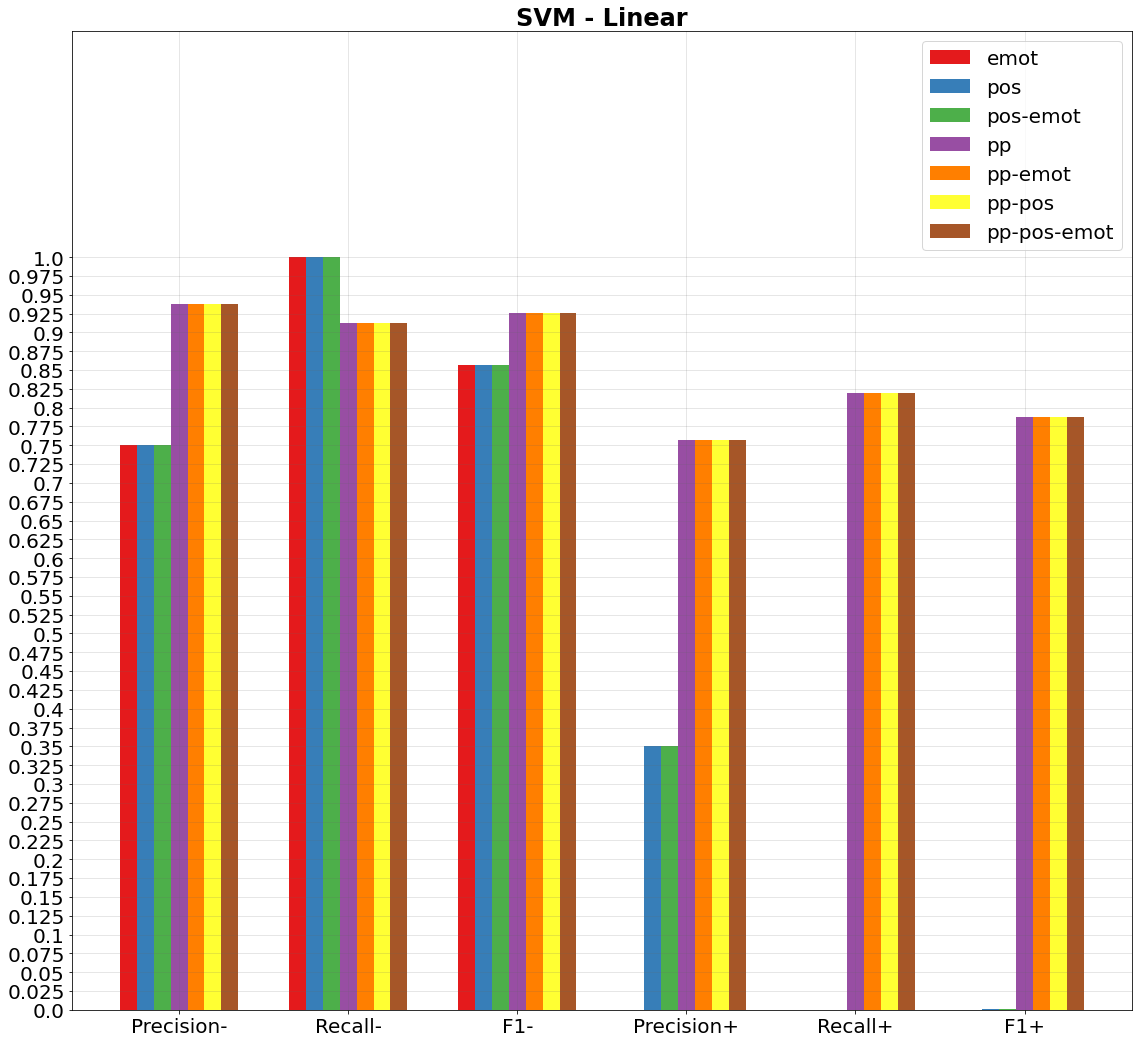
\includegraphics[width=10cm]{assets/reports/micro/nobow/SVM - Linear.png}
	\end{subfigure}
\end{figure}

\vfill
\restoregeometry

\newpage
\newgeometry{
	bottom=0cm
}
\subsubsection{Confusion matrix}


\begin{figure}[H]
	\centering
	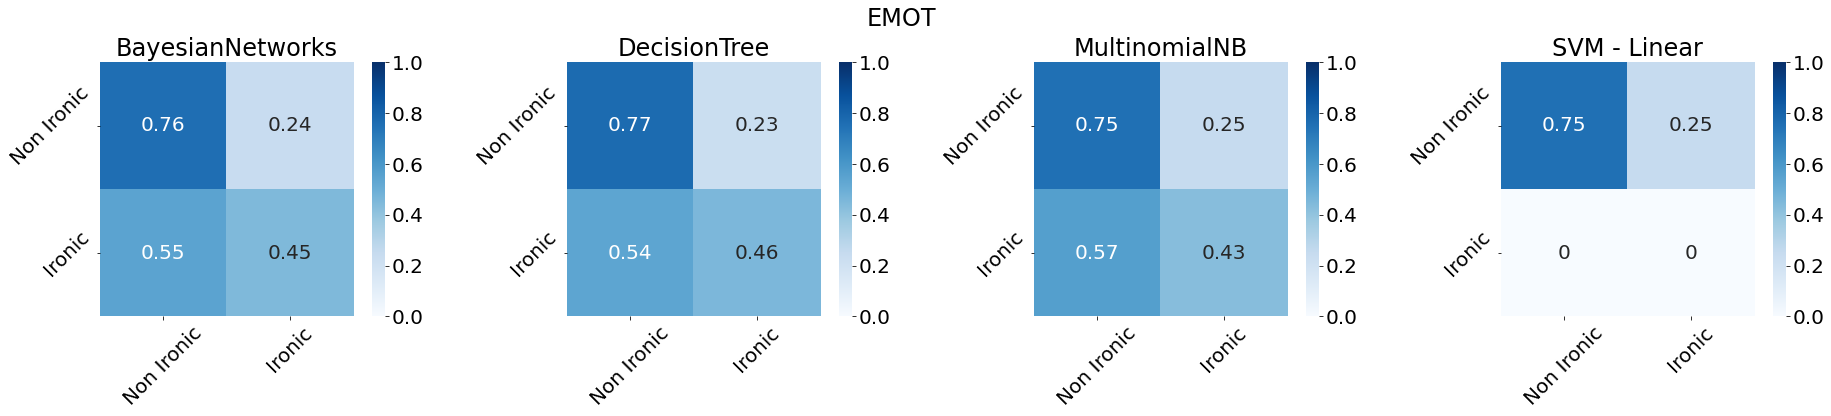
\includegraphics[width=13cm]{assets/reports/conf-matrix/nobow/emot.png}
\end{figure}
\vspace*{-0.8cm}

\begin{figure}[H]
	\centering
	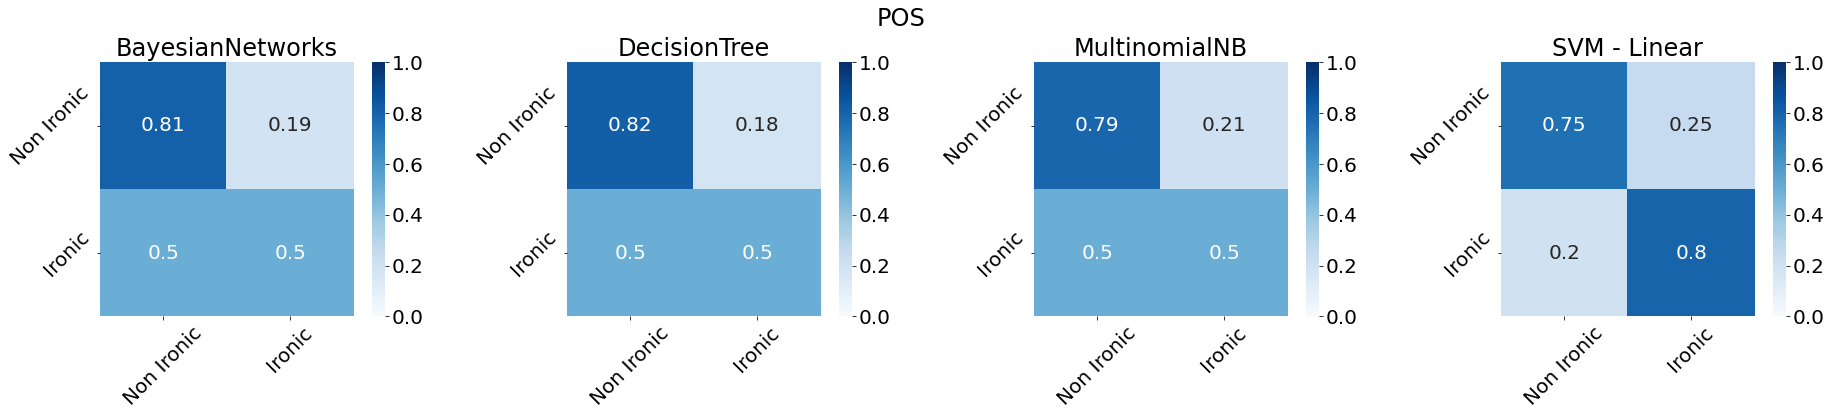
\includegraphics[width=13cm]{assets/reports/conf-matrix/nobow/pos.png}
\end{figure}
\vspace*{-0.8cm}

\begin{figure}[H]
	\centering
	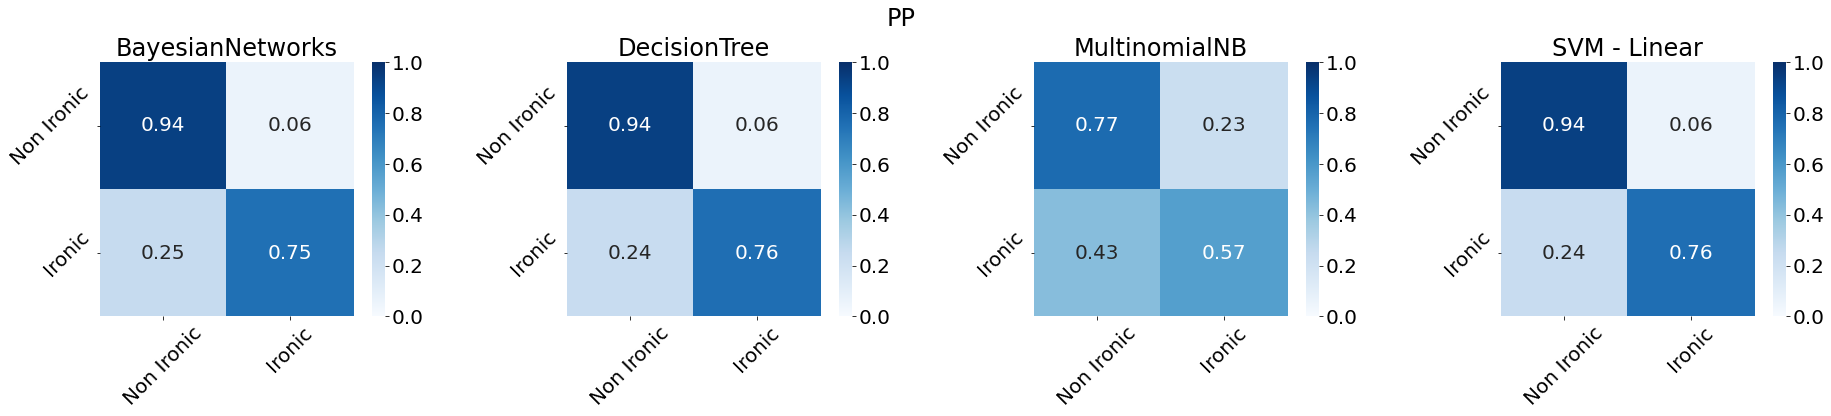
\includegraphics[width=13cm]{assets/reports/conf-matrix/nobow/pp.png}
\end{figure}
\vspace*{-0.8cm}

\begin{figure}[H]
	\centering
	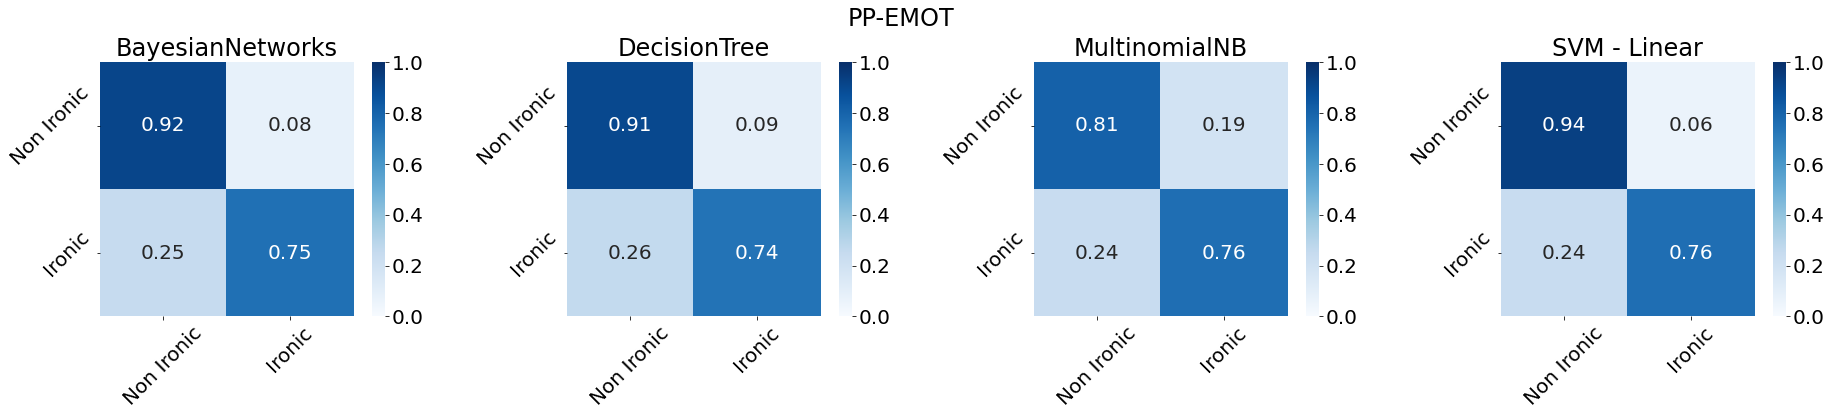
\includegraphics[width=13cm]{assets/reports/conf-matrix/nobow/pp-emot.png}
\end{figure}
\vspace*{-0.8cm}

\begin{figure}[H]
	\centering
	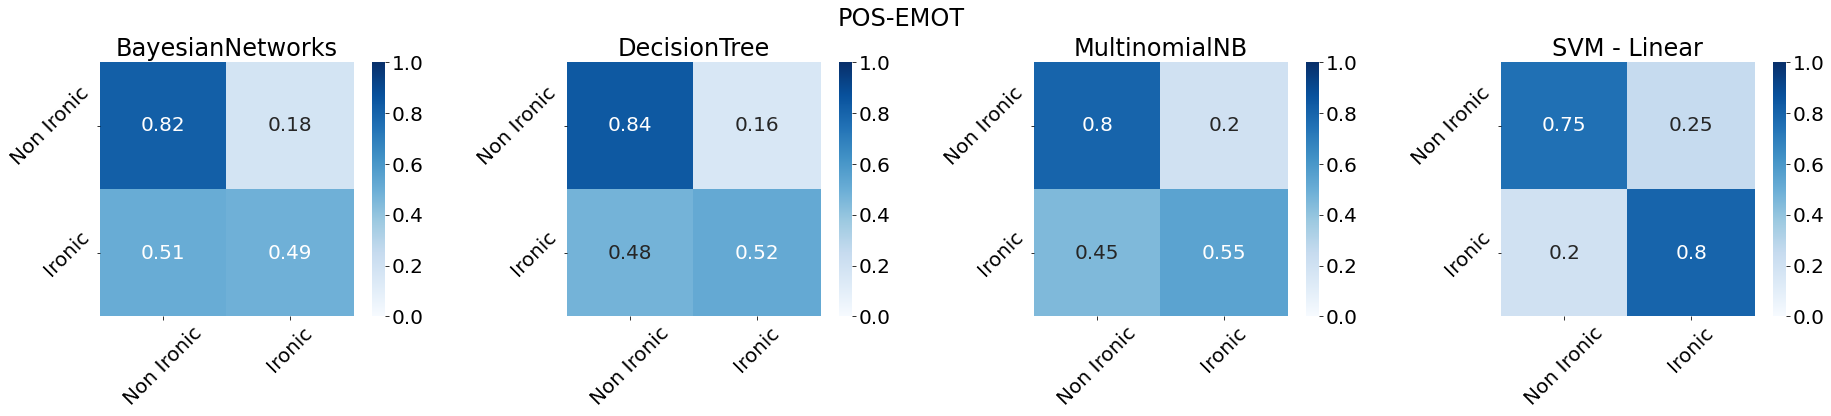
\includegraphics[width=13cm]{assets/reports/conf-matrix/nobow/pos-emot.png}
\end{figure}
\vspace*{-0.8cm}

\begin{figure}[H]
	\centering
	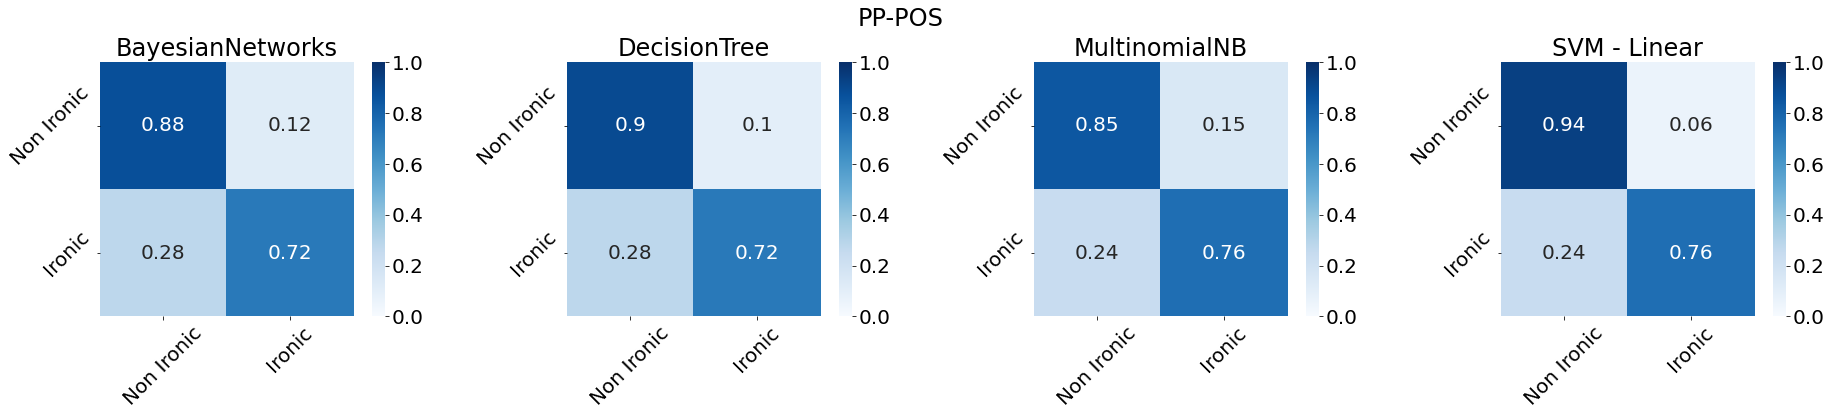
\includegraphics[width=13cm]{assets/reports/conf-matrix/nobow/pp-pos.png}
\end{figure}
\vspace*{-0.8cm}

\begin{figure}[H]
	\centering
	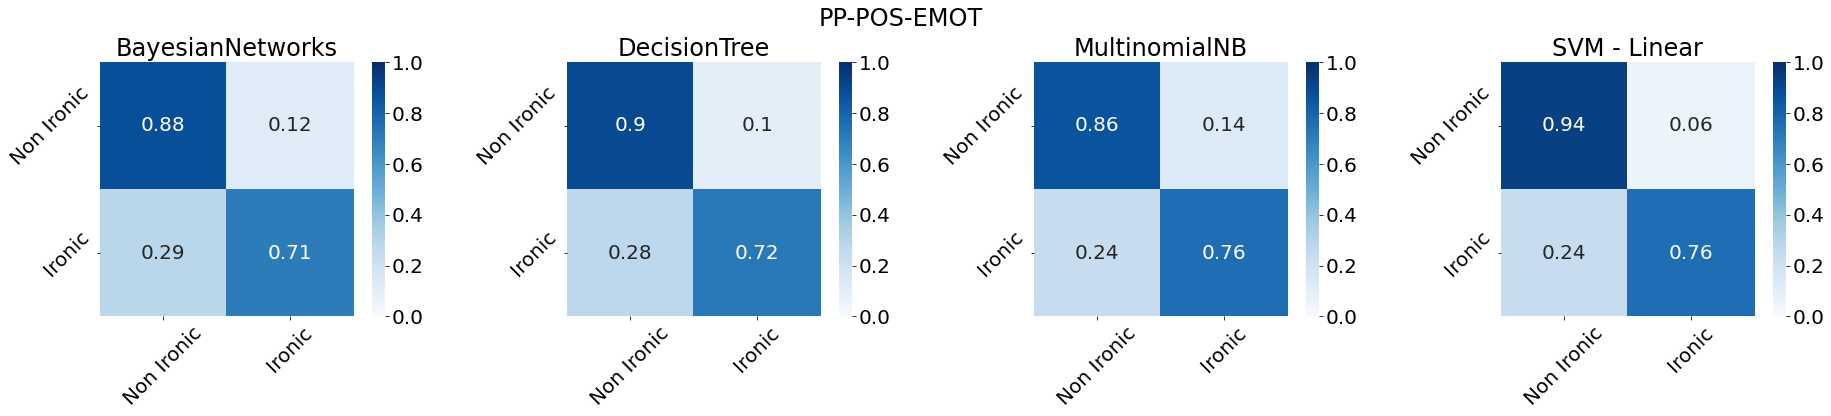
\includegraphics[width=13cm]{assets/reports/conf-matrix/nobow/pp-pos-emot.png}
\end{figure}
\vspace*{-0.8cm}
\restoregeometry
\newpage

\subsubsection{Osservazioni}
In questi esperimenti non viene considerata la rappresentazione del testo come feature. Le performance migliori si ottengono con l'algoritmo decision tree considerando solo le features relative alle particelle pragmatiche (F1 = 0.8898).

I risultati mostrano come, per ogni classificatore, solo le features relative alle emozioni sono le peggiori per classificare i tweets. Tuttavia questa informazione, se combinata con altre features, risulta essere utile per migliorare le performance. Dagli esperimenti emerge inoltre come la feature più importante per distinguere da sola l'ironia sia quella relativa alla particelle pragmatiche, quindi punteggiature, emoticons, acronomi e espressioni onomatopeiche. Si noti come, in effetti, l'uso di emoticons in particolare, ma più in generale delle particelle pragmatiche, sono un importante strumento per esprimere le emozioni, ed esse trasportano un'importante componente emotiva intrinseca.

Nel caso dell'algoritmo SVM, utilizzando esclusivamente features come emotion e POS tags, si raggunge l'accuracy del 75\%. Tuttavia questo è un chiaro esempio di come una metrica F1 sia decisamente più affidabile per valutare le performance di un classificatore. Infatti considerando il caso dell'algoritmo SVM e la feature emotion, analizzando il risultato della classificazione solo per la classe positiva (quella ironica) si ha un il recall pari a 0. Questo dato emerge anche dalla relativa matrice di confusione, infatti si evince chiaramente come i documenti vengano classificati tutti come non ironici. Questo è coerente con l'accuracy al 75\%, essendo il dataset composto per $\frac{3}{4}$ da messaggi non ironici e $\frac{1}{4}$ da messaggi ironici.




\newpage
\subsection{BOW + Caratteristiche linguistiche}

\subsubsection{Weighted average}
\vfill
\begin{figure}[!h]
	\hspace*{-3cm}
	\begin{subfigure}[b]{0.5\textwidth}
		\centering
		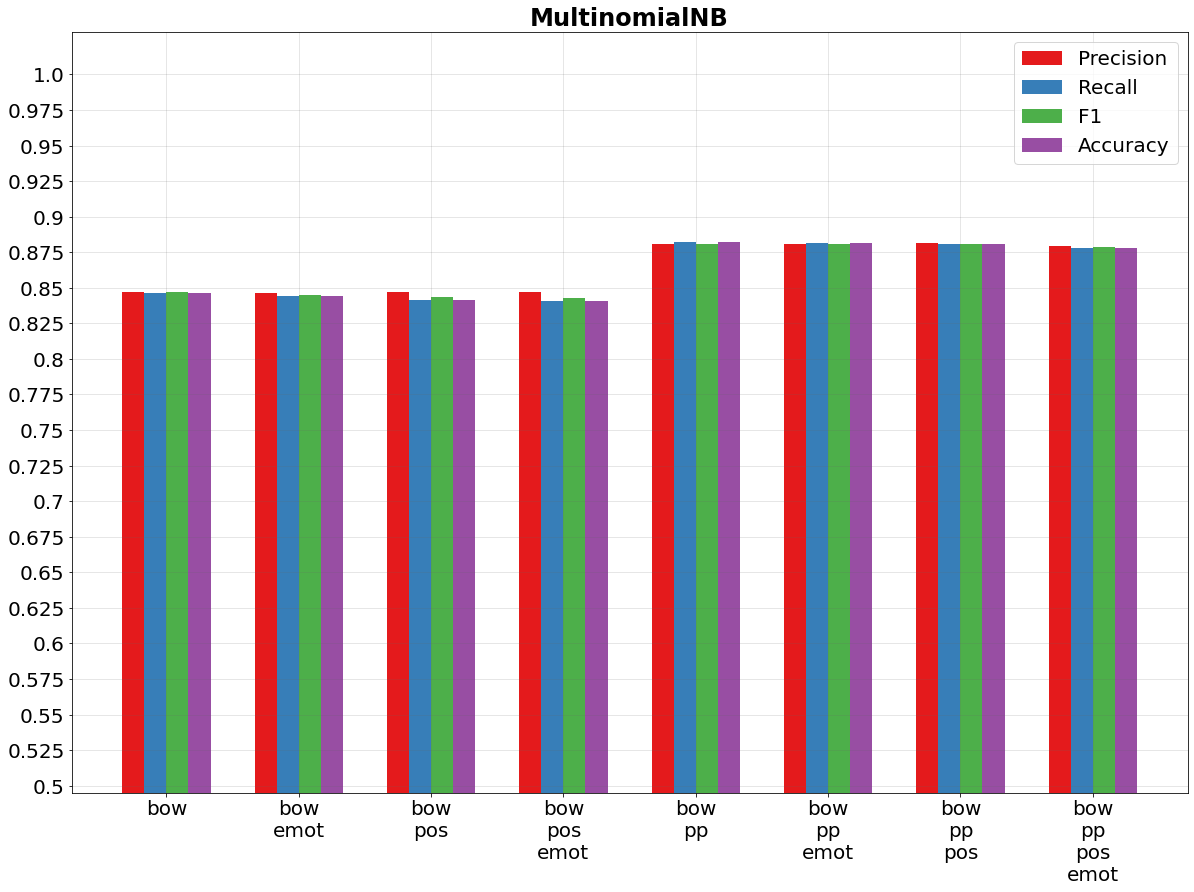
\includegraphics[width=10cm]{assets/reports/macro/bow/MultinomialNB.png}
	\end{subfigure}
	\hfill
	\begin{subfigure}[b]{0.5\textwidth}
		\centering
		\hspace*{0.15cm}
		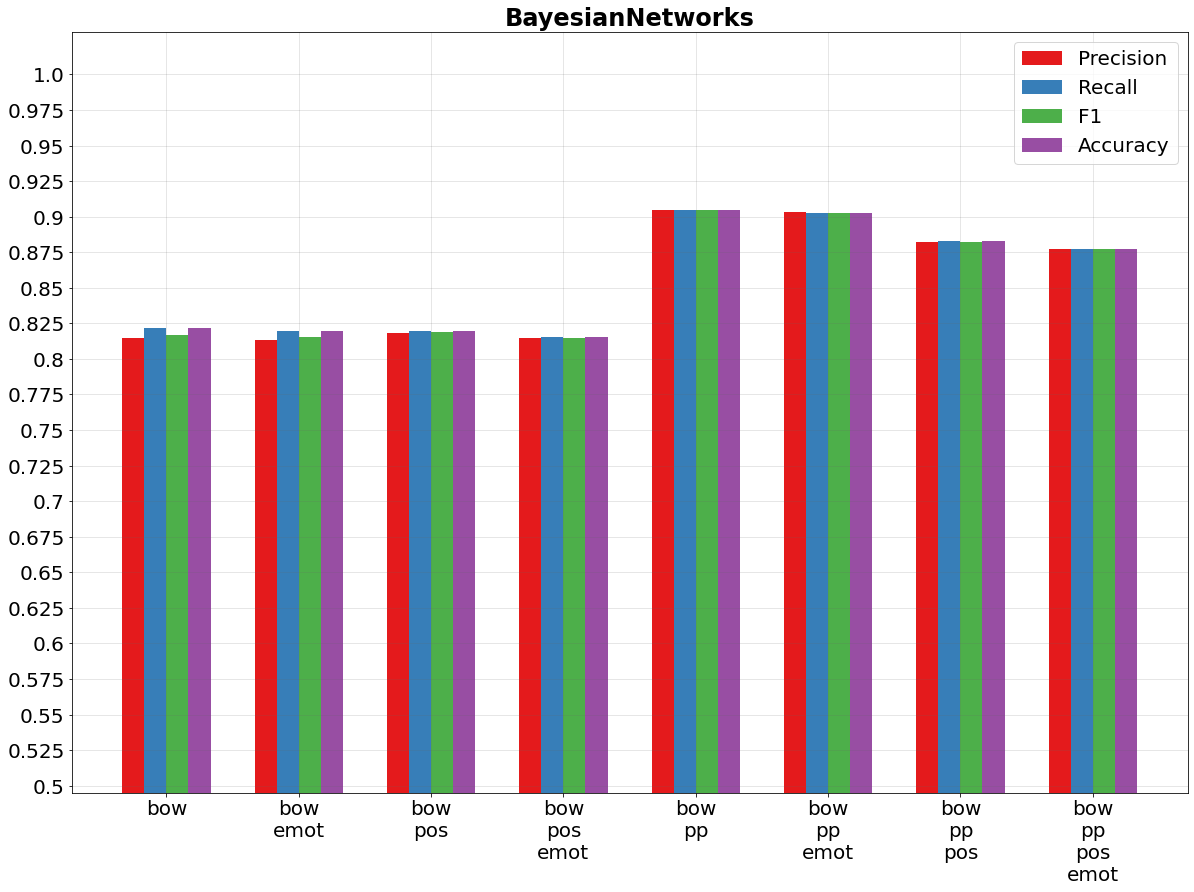
\includegraphics[width=10cm]{assets/reports/macro/bow/BayesianNetworks.png}
	\end{subfigure}
\end{figure}
\vfill
\begin{figure}[!h]
	\hspace*{-3cm}
	\begin{subfigure}[b]{0.5\textwidth}
		\centering
		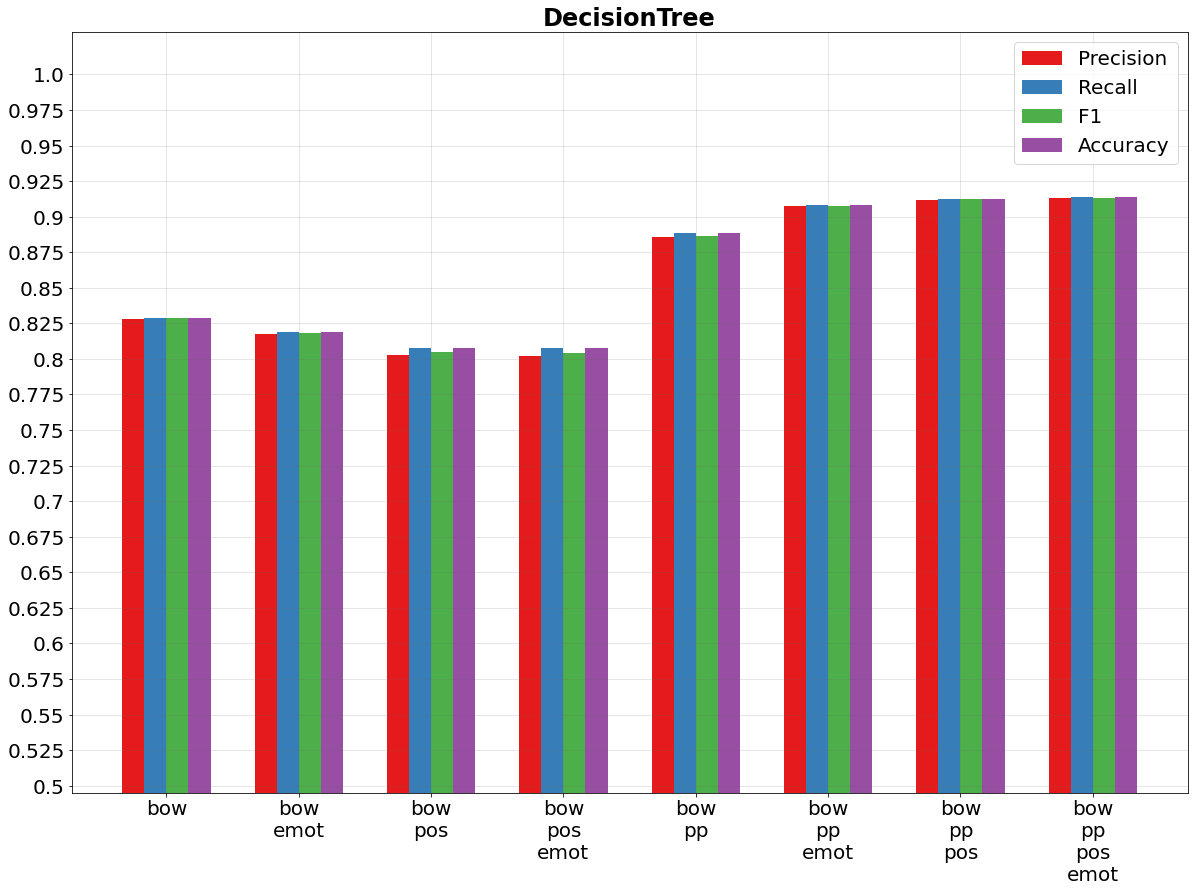
\includegraphics[width=10cm]{assets/reports/macro/bow/DecisionTree.png}
	\end{subfigure}
	\hfill
	\begin{subfigure}[b]{0.5\textwidth}		
		\centering
		\hspace*{0.15cm}
		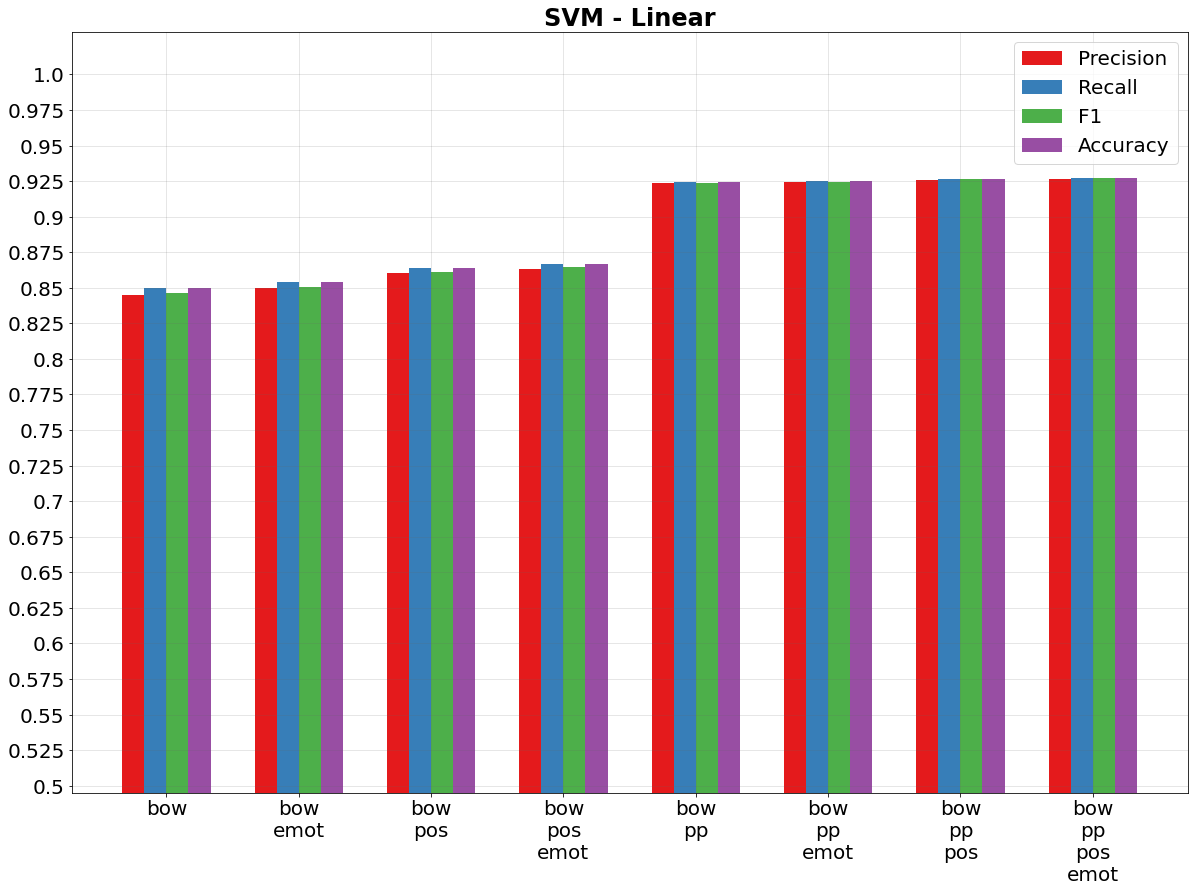
\includegraphics[width=10cm]{assets/reports/macro/bow/SVM - Linear.png}
	\end{subfigure}
\end{figure}
\newpage

\begin{figure}[!h]
	\hspace*{-3cm}
	\begin{subfigure}[b]{0.5\textwidth}
		\centering
		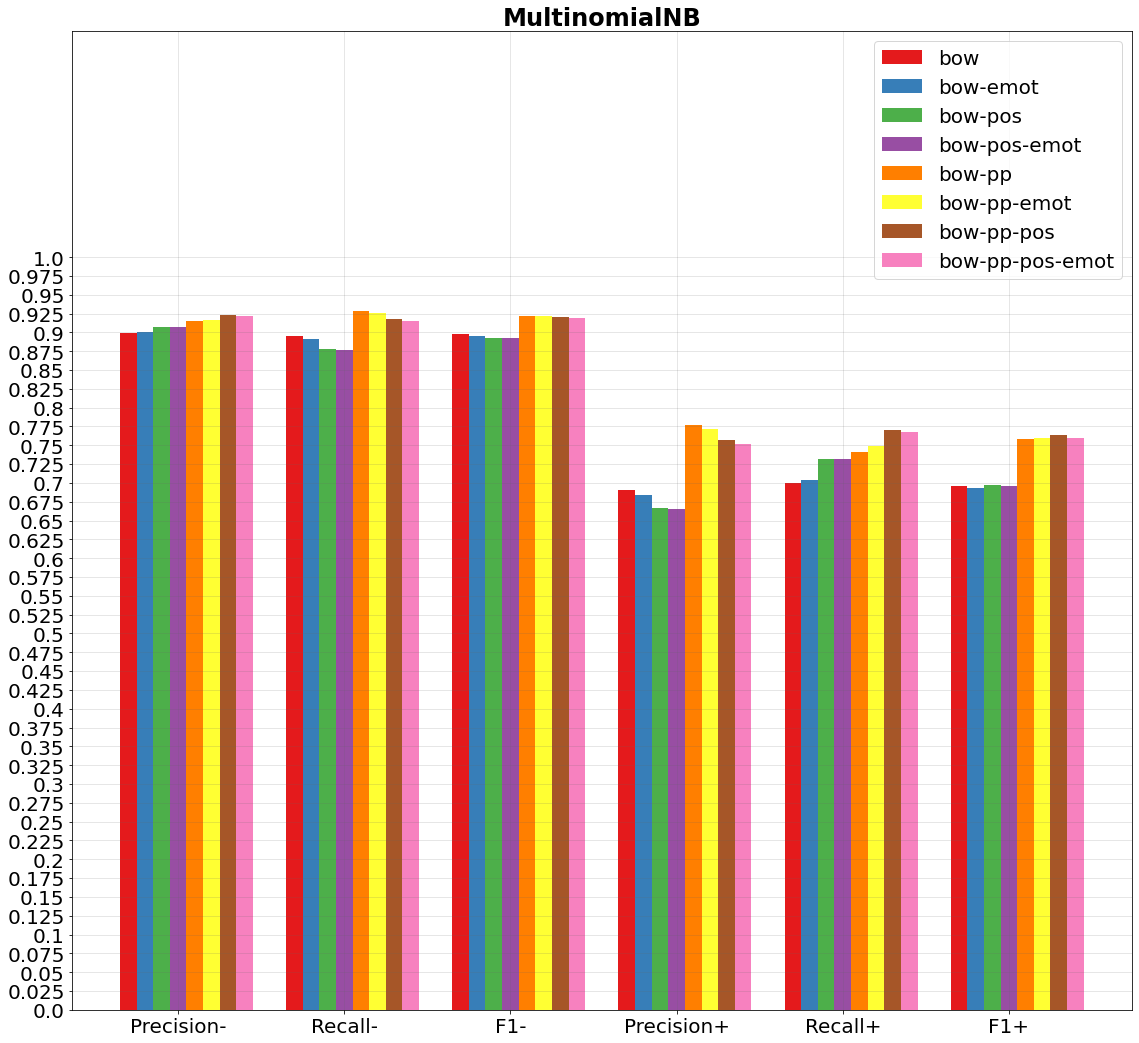
\includegraphics[width=10cm]{assets/reports/micro/bow/MultinomialNB.png}
	\end{subfigure}
	\hfill
	\begin{subfigure}[b]{0.5\textwidth}
		\hspace*{0.15cm}
		\centering
		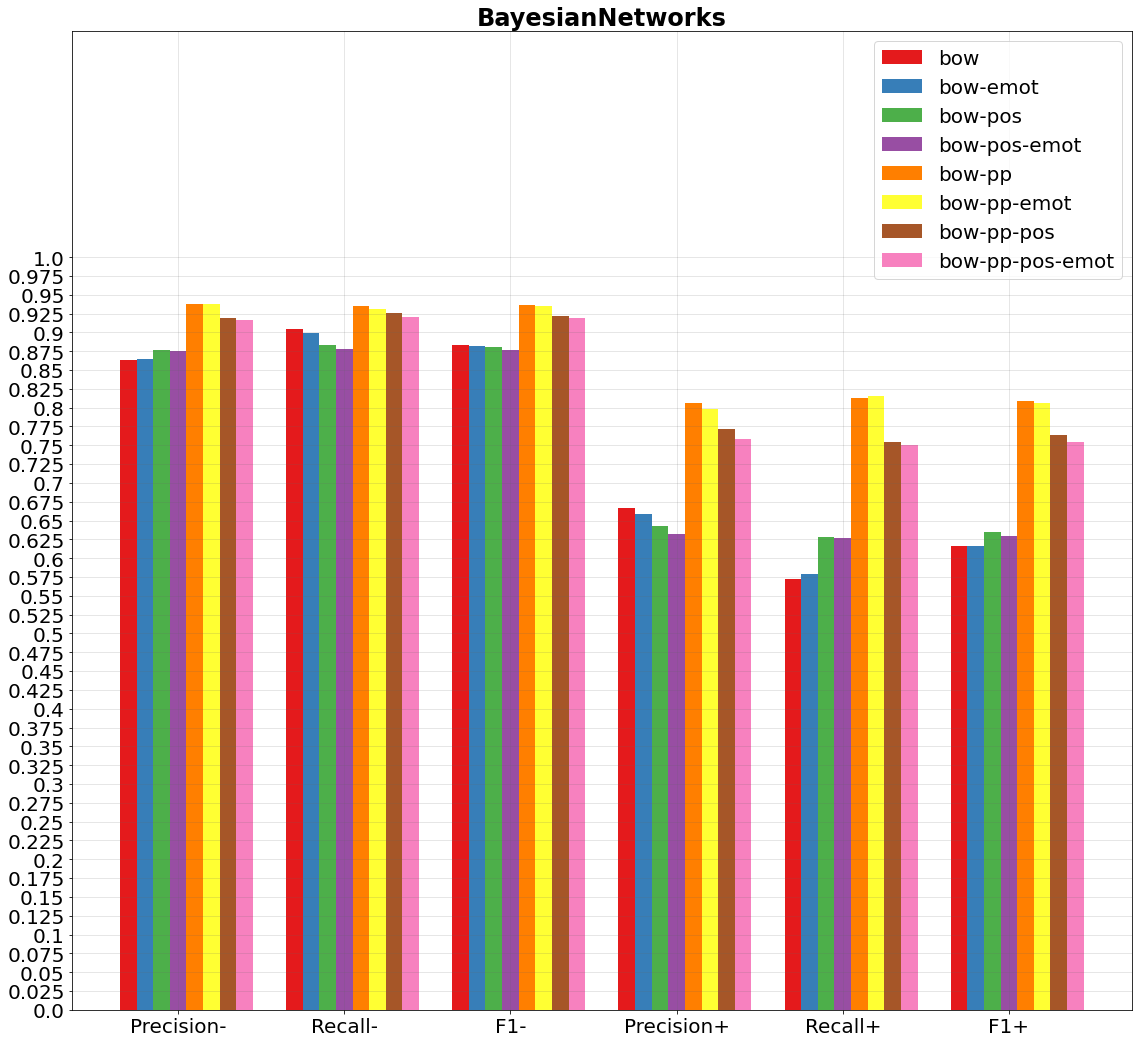
\includegraphics[width=10cm]{assets/reports/micro/bow/BayesianNetworks.png}
	\end{subfigure}
\end{figure}
\vfill
\begin{figure}[!h]
	\hspace*{-3cm}
	\begin{subfigure}[b]{0.5\textwidth}
		\centering
		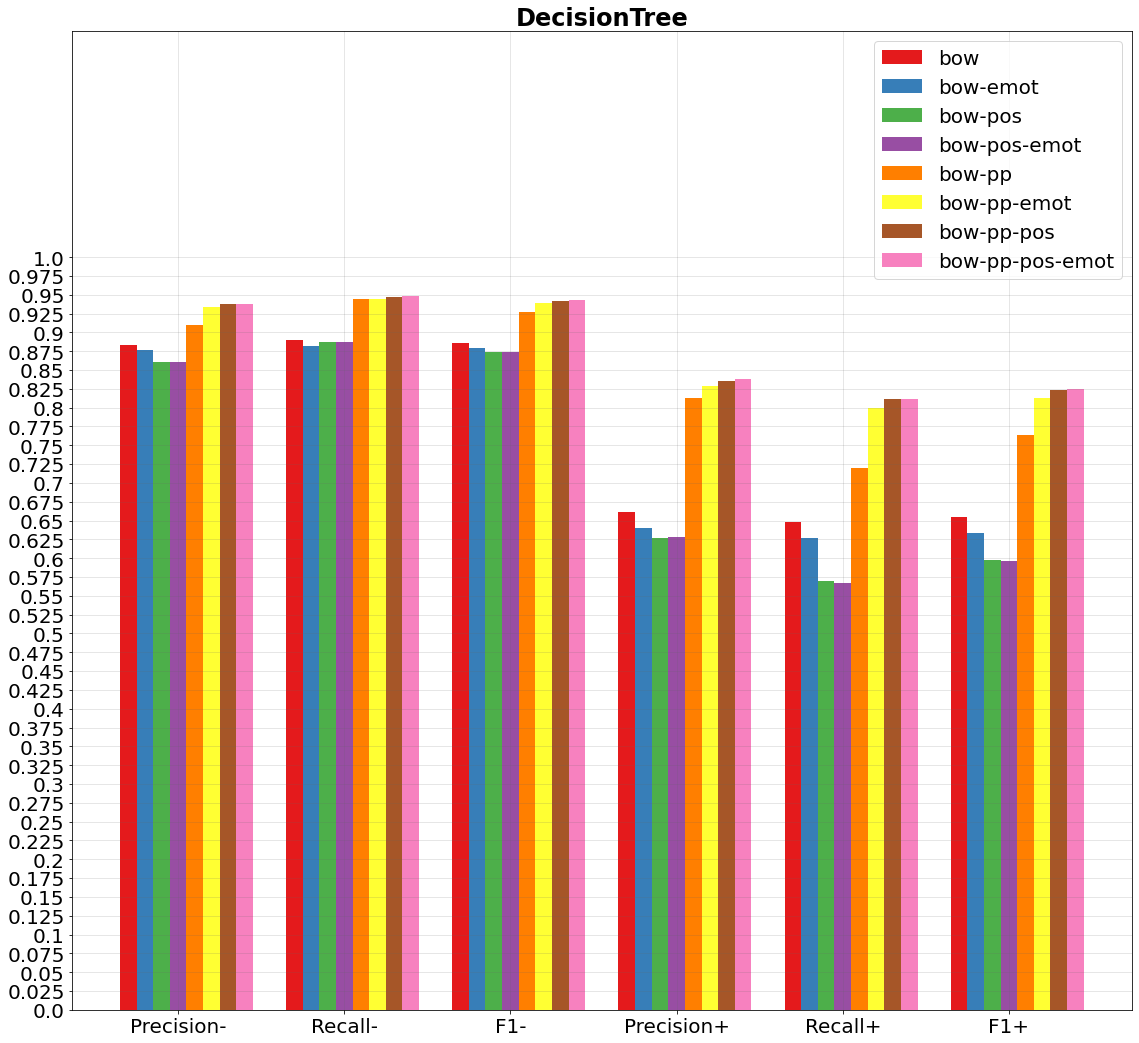
\includegraphics[width=10cm]{assets/reports/micro/bow/DecisionTree.png}
	\end{subfigure}
	\hfill
	\begin{subfigure}[b]{0.5\textwidth}
		\centering
		\hspace*{0.15cm}
		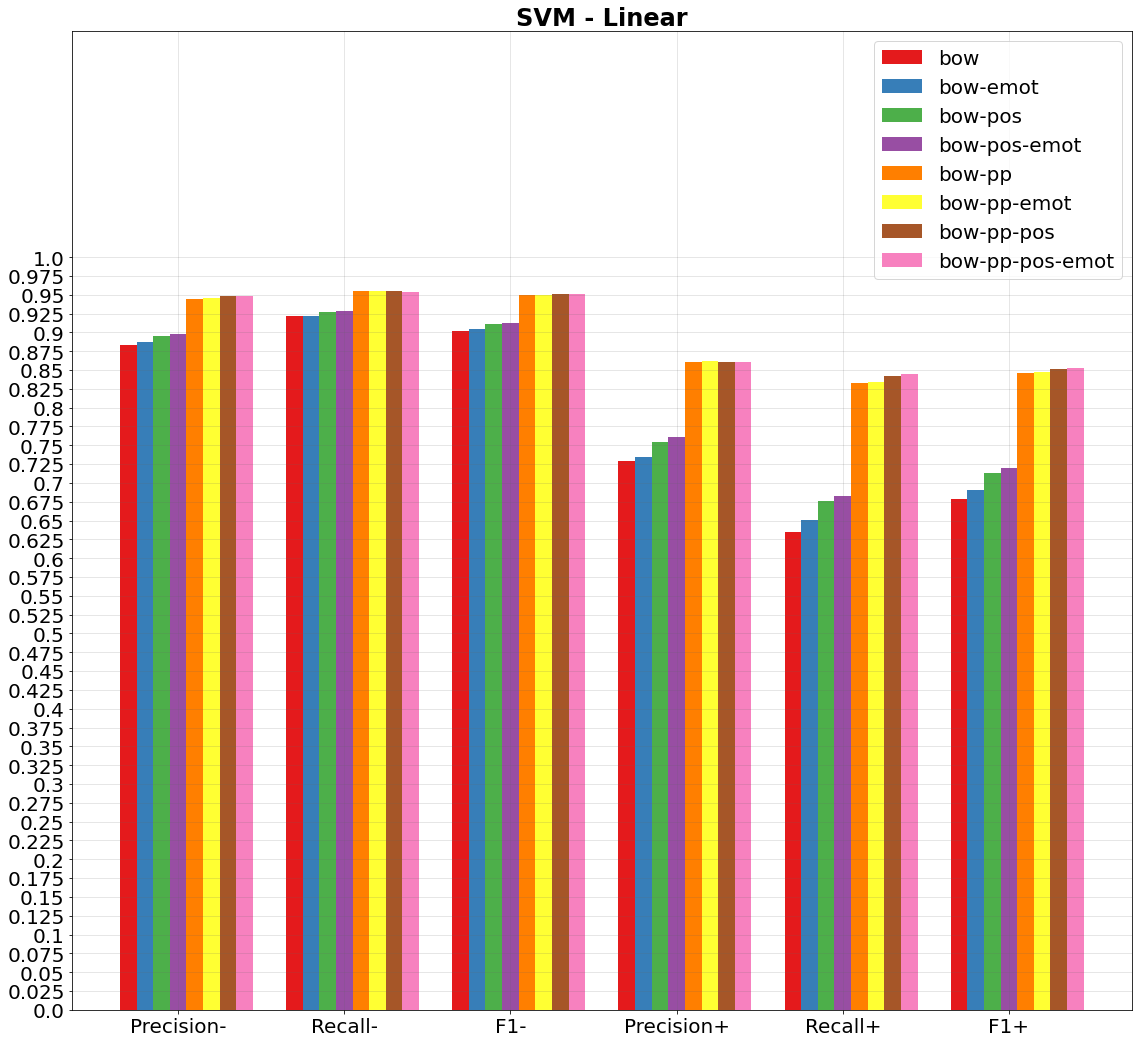
\includegraphics[width=10cm]{assets/reports/micro/bow/SVM - Linear.png}
	\end{subfigure}
\end{figure}

\vfill
\restoregeometry

\newpage
\newgeometry{
	bottom=0cm
}
\subsubsection{Confusion matrix}


\begin{figure}[H]
	\centering
	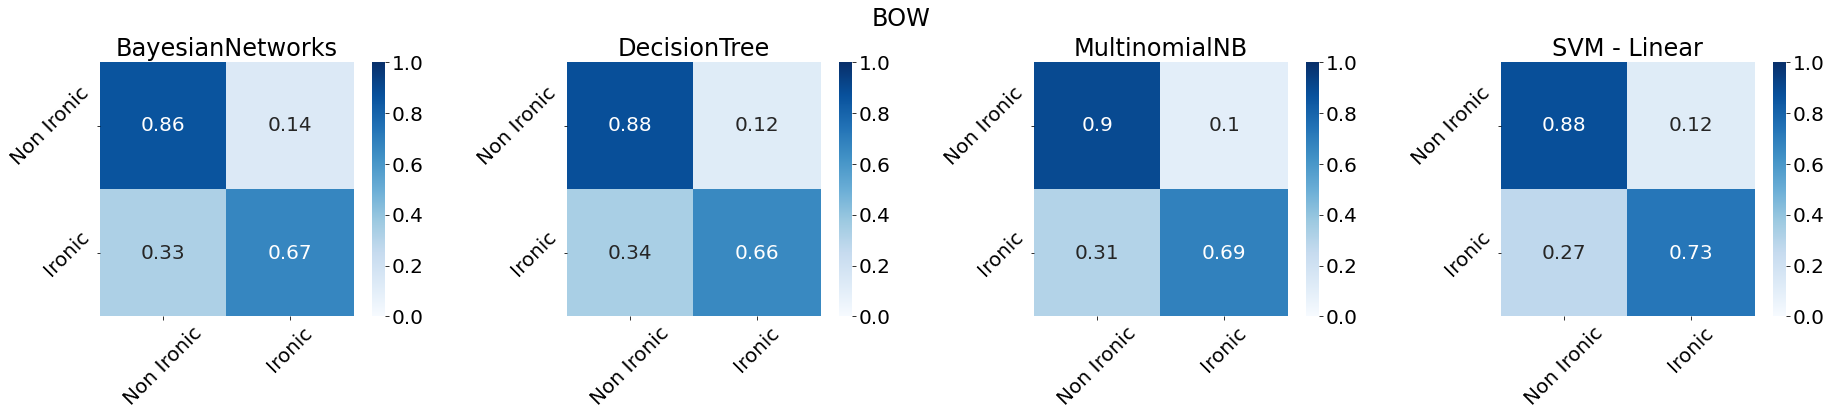
\includegraphics[width=13cm]{assets/reports/conf-matrix/bow/bow.png}
\end{figure}
\vspace*{-0.8cm}

\begin{figure}[H]
	\centering
	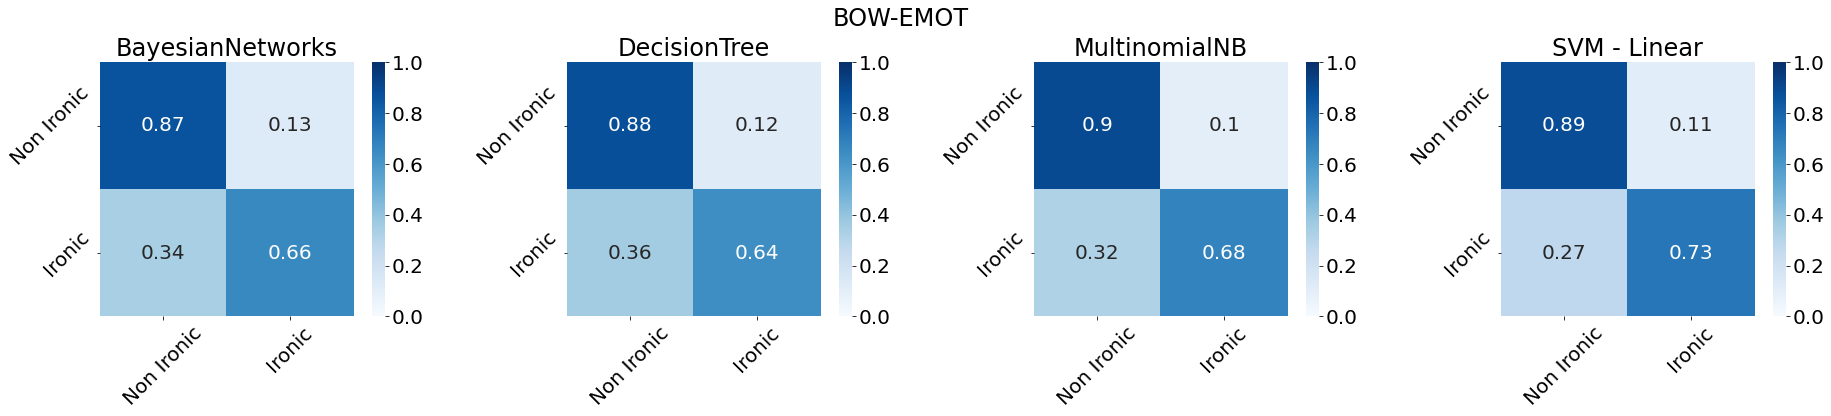
\includegraphics[width=13cm]{assets/reports/conf-matrix/bow/bow-emot.png}
\end{figure}
\vspace*{-0.8cm}

\begin{figure}[H]
	\centering
	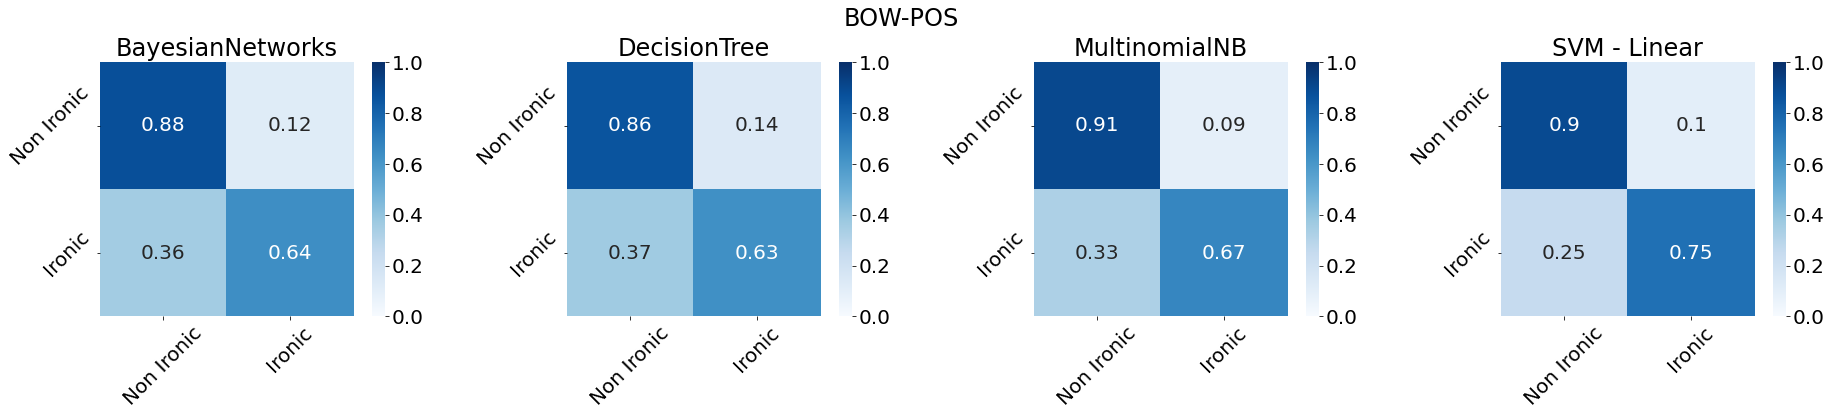
\includegraphics[width=13cm]{assets/reports/conf-matrix/bow/bow-pos.png}
\end{figure}
\vspace*{-0.8cm}

\begin{figure}[H]
	\centering
	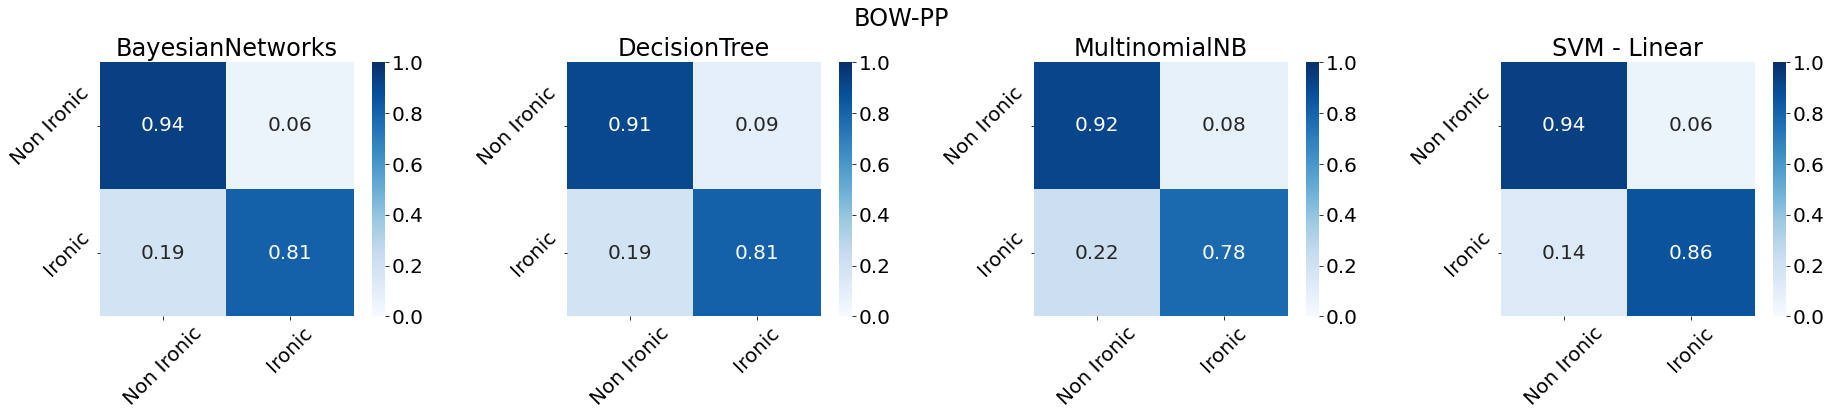
\includegraphics[width=13cm]{assets/reports/conf-matrix/bow/bow-pp.png}
\end{figure}
\vspace*{-0.8cm}

\begin{figure}[H]
	\centering
	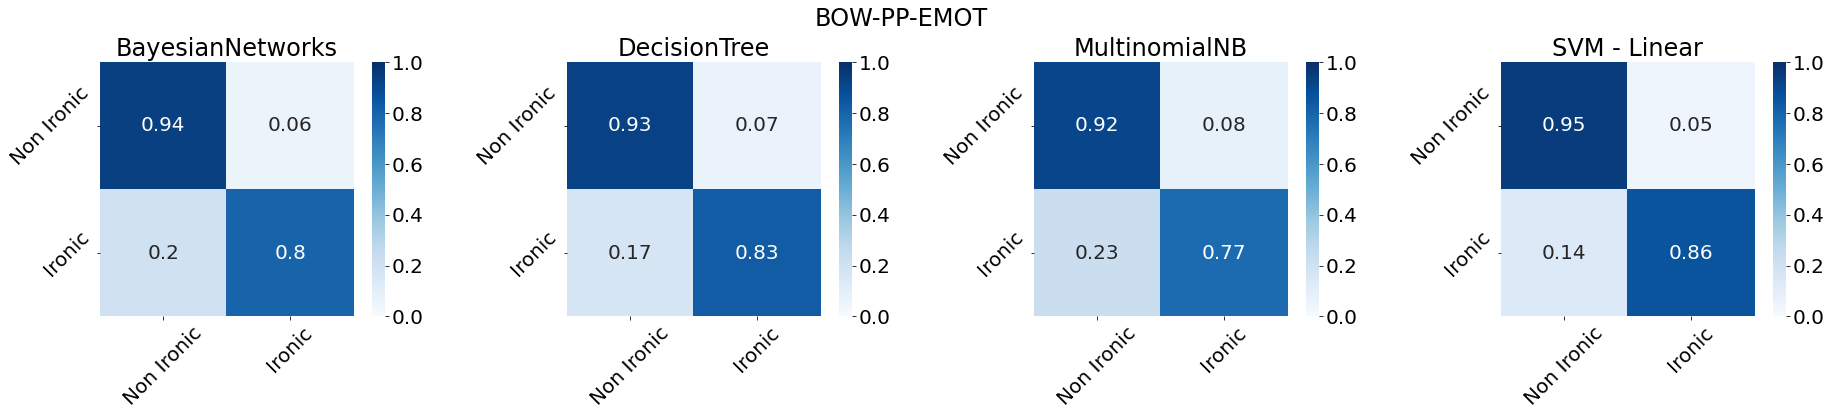
\includegraphics[width=13cm]{assets/reports/conf-matrix/bow/bow-pp-emot.png}
\end{figure}
\vspace*{-0.8cm}

\begin{figure}[H]
	\centering
	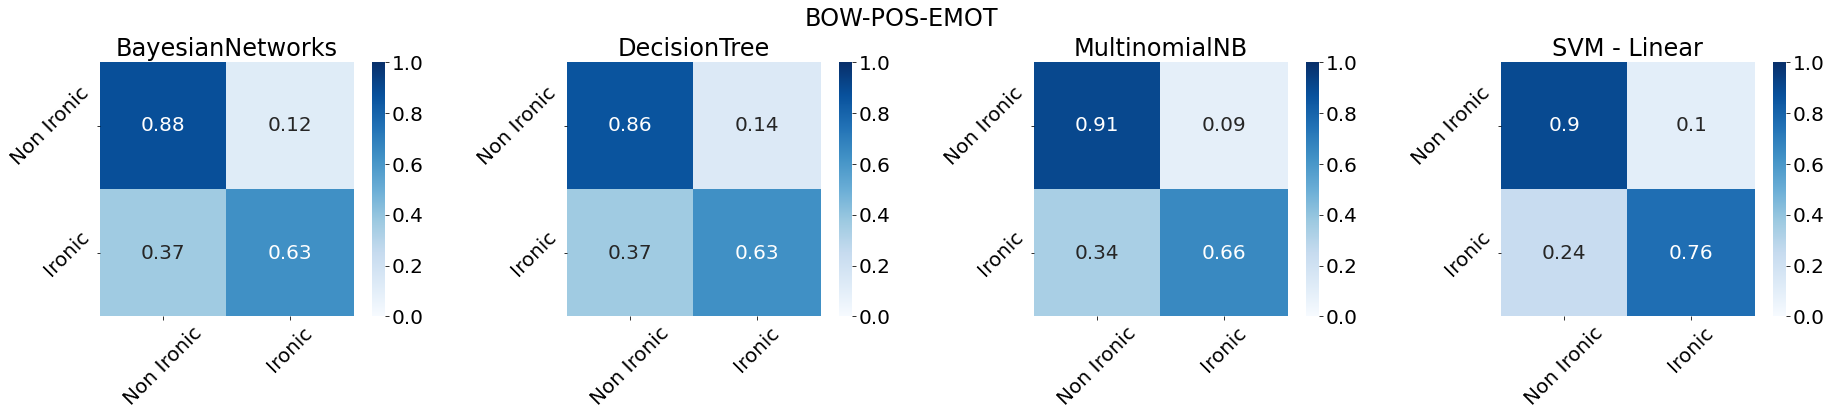
\includegraphics[width=13cm]{assets/reports/conf-matrix/bow/bow-pos-emot.png}
\end{figure}
\vspace*{-0.8cm}

\begin{figure}[H]
	\centering
	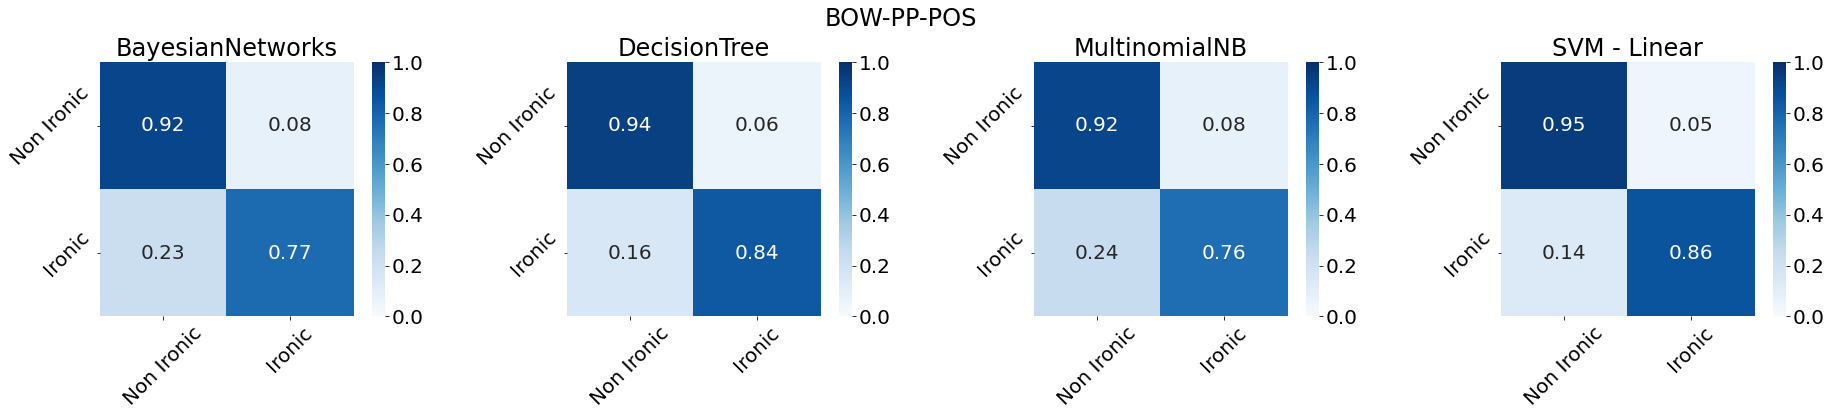
\includegraphics[width=13cm]{assets/reports/conf-matrix/bow/bow-pp-pos.png}
\end{figure}
\vspace*{-0.8cm}

\begin{figure}[H]
	\centering
	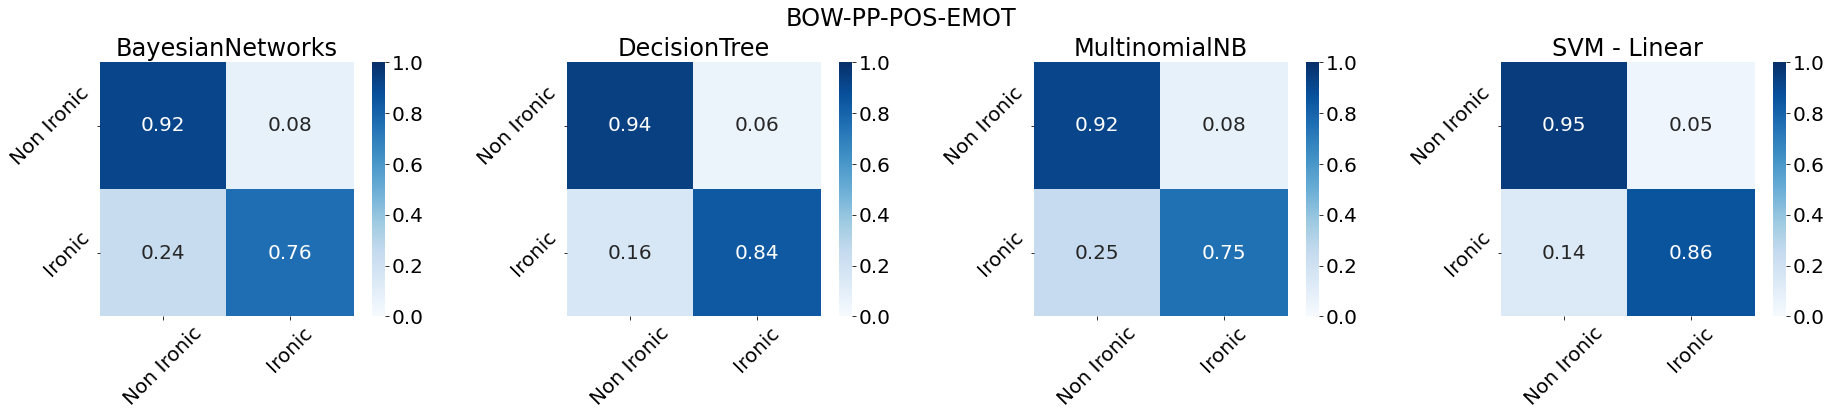
\includegraphics[width=13cm]{assets/reports/conf-matrix/bow/bow-pp-pos-emot.png}
\end{figure}
\vspace*{-0.8cm}
\restoregeometry
\newpage
\subsubsection{Osservazioni}
In questi esperimenti, oltre alle features linguistiche, si utilizza la tecnica BOW per rappresentare il testo. L'algoritmo SVM che prende in input tutte le features estratte, ottiene le performance migliori in assoluto tra tutti i modelli considerati (Accuracy = 0.9270, F1 = 0.9268).

Anche per quanto riguarda riconoscere i tweets ironici, considerando l'algoritmo SVM e tenendo conto di tutte le features, analizzando i reports relativi solamente alla classe positiva, e basandosi sia sul recall che sulla metrica F1, si può vedere come in questo modo si ottengono le performance migliori rispetto ad altri classificatori e diverse features.

Inoltre, come negli esperimenti precedenti, si può notare come features relative alle particelle pragmatiche forniscono un netto miglioramento nelle performance.

\newpage

\subsection{BOW vs BERT vs Sentence-BERT}

\subsubsection{Weighted average - Accuracy}

\begin{figure}[!h]
	\hspace*{-3cm}
	\begin{subfigure}[b]{0.5\textwidth}
		\centering
		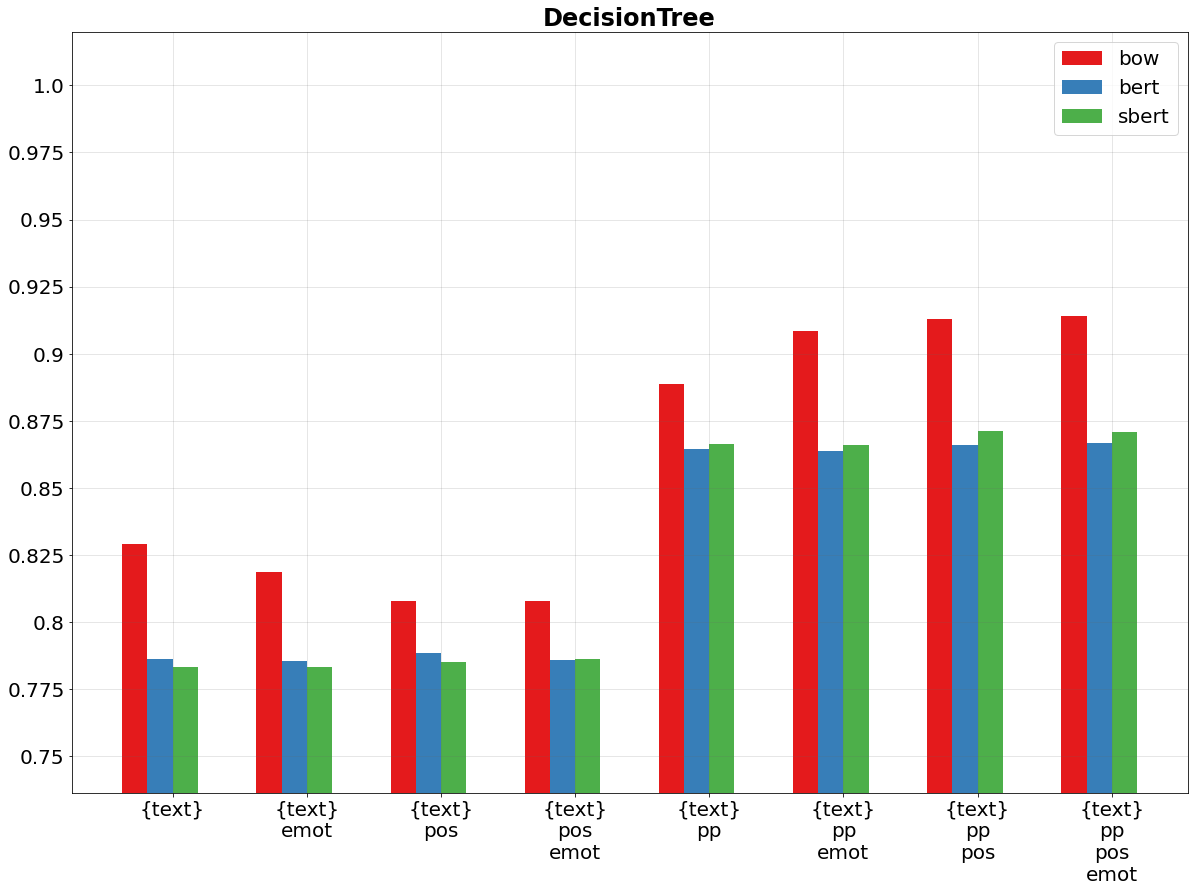
\includegraphics[width=10cm]{assets/reports/text/acc/DecisionTree.png}
	\end{subfigure}
	\hfill
	\begin{subfigure}[b]{0.5\textwidth}		
		\centering
		\hspace*{0.15cm}
		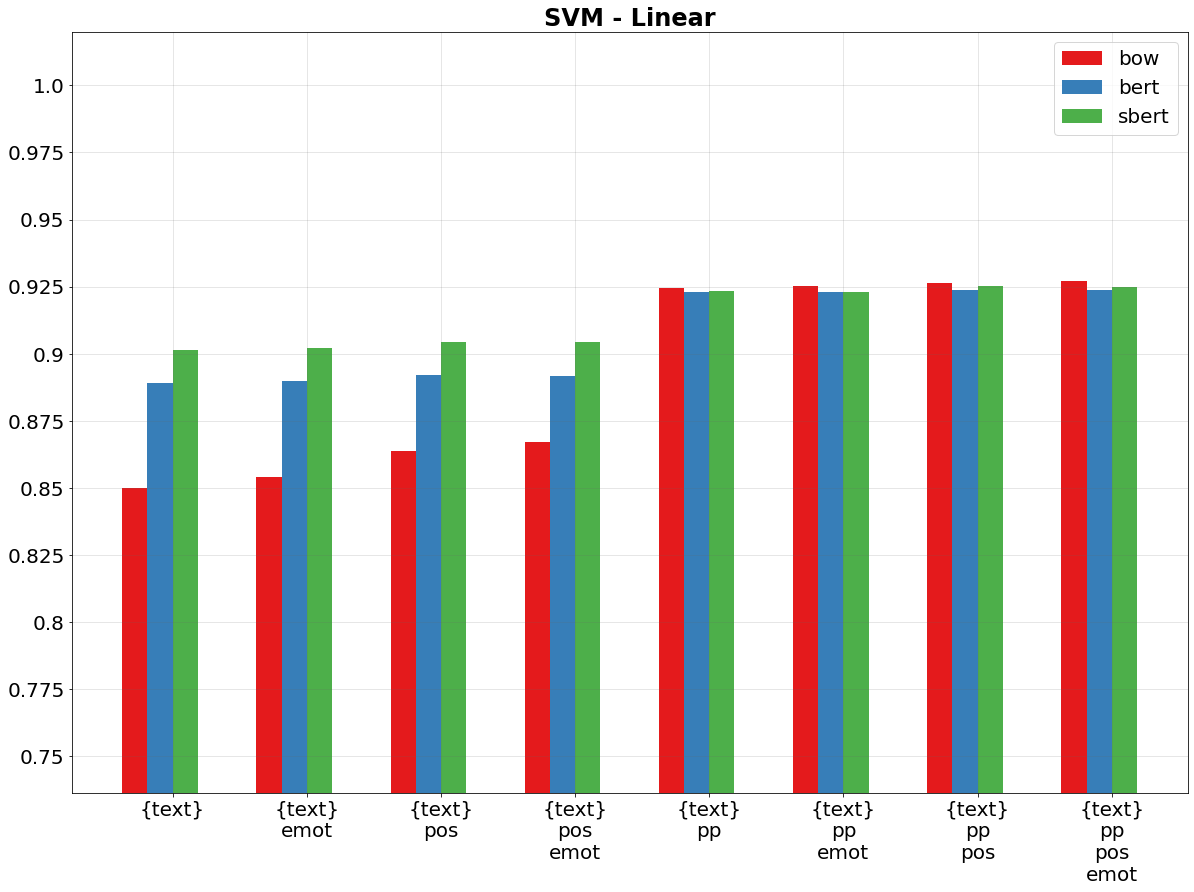
\includegraphics[width=10cm]{assets/reports/text/acc/SVM - Linear.png}
	\end{subfigure}
\end{figure}
\subsubsection{Weighted average - F measure}

\begin{figure}[!h]
	\hspace*{-3cm}
	\begin{subfigure}[b]{0.5\textwidth}
		\centering
		\includegraphics[width=10cm]{assets/reports/text/f1/DecisionTree.png}
	\end{subfigure}
	\hfill
	\begin{subfigure}[b]{0.5\textwidth}		
		\centering
		\hspace*{0.15cm}
		\includegraphics[width=10cm]{assets/reports/text/f1/SVM - Linear.png}
	\end{subfigure}
\end{figure}
\newpage


\subsubsection{Osservazioni}
In questi esperimenti vengono messe a confronto diverse tecniche per la rappresentazione del testo. Analizzando i reports ottenuti, possiamo notare come le performance migliori si ottengono anche in questo caso considerando la rappresentazione del testo BOW con tutte le features aggiuntive. Si tenga presente che l'algoritmo decision tree, tende ad andare in overfitting, si ritiene pertanto il risultato ottenuto da SVM più affidabile.

Si può notare come effettivamente considerando la rappresentazione mediante Sentece-BERT, le performance migliorano leggermente rispetto che adottare una semplice pooling strategy con BERT. Inoltre finché non si prendono in considerazione le features relative alle particelle pragmatiche, le performance rimangono pressoché uguali. Questo è dato dal fatto che sia BERT che Sentece-BERT generano embeddings tenendo conto della semantica assunta dal token all'interno della frase, quindi informazioni utili fornite dai POS tags riguardo la sintassi, in questo caso sono meno sfruttate, a differenza di una rappresentazione BOW.


\newpage

\subsection{Analisi lessico con PCA}
La principal component analysis (PCA) è una tecnica per la semplificazione dei dati, il cui scopo è ridurre il numero di variabili che descrivono il dataset, limitando il più possibile la perdita di informazioni.

Per limitare la perdita di informazioni, si considerano solo quelle variabili con la quantità di varianza spiegata più alta, ovvero quelle che meglio differenziano il dataset, per l'appunto le componenti principali. Di fatto la riduzione delle dimensioni sfrutta questo aspetto, ma nel caso considerato si terrà conto solo del contributo di ogni variabile, senza realmente andare a ridurre le dimensioni del dataset.

A questo scopo si procede standardizzando il dataset, quindi viene calcolata la matrice di covarianza $n \times n$ dove $n$ corrisponde al numero di variabili. Dopodiché si calcolano gli autovalori associati agli autovettori della matrice di covarianza. Come risultato si ottengono le componenti principali, nuove variabili costruite come combinazione lineare delle variabili di partenza. La percentuale di varianza spiegata da ogni componente principale si calcola a partire dagli autovalori: $$\%PC_k = \frac{\lambda_k}{\sum_{i=1}^n \lambda_i}$$

Questa tecnica viene qui utilizzata per analizzare il lessico e cercare un'eventuale associazione tra parole e ironia. Si considera quindi il dataset ironico e non ironico separatamente, e si procede generando gli embeddings tramite BERT. Si ottiene la matrice $M$ composta dagli embeddings sulle colonne, e le diverse parole che occorrono nel dataset sulle righe. Dal momento che si vuole cercare un'associazione tra le parole e l'ironia, si considera la matrice $M^T$ e si effettua PCA, così da valutare se alcune parole contribuiscono maggiormente relativamente al dataset ironico.

\subsubsection{Top k componenti principali}
Per ogni componente principale, viene calcolata la varianza spiegata. Di seguito viene mostrata la varianza spiegata dalle prime 50 componenti principali (la varianza spiegata totale è 1):

\begin{figure}[H]
	\begin{subfigure}[H]{0.5 \textwidth}
		\centering
		\includegraphics[width=7.25cm]{assets/pca/non_ironic/var.png}
		\caption{Dataset non ironico}
	\end{subfigure}
	\hfill
	\begin{subfigure}[H]{0.5 \textwidth}
		\centering
		\includegraphics[width=7.25cm]{assets/pca/ironic/var.png}
		\caption{Dataset ironico}
	\end{subfigure}
	\caption{Varianza spiegata}
\end{figure}

\begin{figure}[H]
	\begin{subfigure}[H]{0.5 \textwidth}
		\centering
		\includegraphics[width=7.25cm]{assets/pca/non_ironic/cum-var.png}
		\caption{Dataset non ironico}
	\end{subfigure}
	\hfill
	\begin{subfigure}[H]{0.5 \textwidth}
		\centering
		\includegraphics[width=7.25cm]{assets/pca/ironic/cum-var.png}
		\caption{Dataset ironico}
	\end{subfigure}
	\caption{Varianza spiegata cumulata}
\end{figure}


\subsubsection{Features con contributo maggiore}
Per calcolare le features più importanti, si considerano gli autovettori associati agli autovalori, si procede quindi sommando tutti gli elementi del vettore in valore assoluto. Il risultato è il contributo espresso da una particolare feature rispetto a tutte le componenti principali (maggiore il valore, più alta l'importanza) \cite{pcaeigenvectors}. Vengono quindi considerate le 50 features con il contributo più alto (il contributo totale è 1):

\begin{figure}[H]
	\begin{subfigure}[H]{0.5 \textwidth}
		\centering
		\includegraphics[width=7.25cm]{assets/pca/non_ironic/contribution.png}
		\caption{Dataset non ironico}
	\end{subfigure}
	\hfill
	\begin{subfigure}[H]{0.5 \textwidth}
		\centering
		\includegraphics[width=7.25cm]{assets/pca/ironic/contribution.png}
		\caption{Dataset ironico}
	\end{subfigure}
	\caption{Contributo dell features}
\end{figure}

\subsubsection{Osservazioni}
Come si può notare da queste analisi, pur considerando le prime 50 componenti principali, viene spiegata solo il 40\% circa della varianza totale. Inoltre per quanto riguarda il contributo di ogni feature, nessuna di queste prevale tra le altre. Questi ragionamenti data-driven mostrano come non ci sia una chiara associazione tra lessico e ironia. In effetti il risultato è coerente con ciò che ci si aspetta, per riconoscere l'ironia non è infatti sufficiente basarsi solo sul lessico utilizzato nella frase.

\chapter{Conclusioni e sviluppi futuri}
I sistemi di sentiment analysis vengono utilizzati per estrarre l'informazione relativa al sentimento e l'opinione espressa in un testo. Nel linguaggio naturale esistono figure retoriche come l'ironia che sono in grado di invertire completamente la polarità di ciò che si esprime, di conseguenza i sistemi di sentiment analysis vengono "ingannati".

In questa tesi sono stati presentati diversi modelli di machine learning supervisionati per il riconoscimento dell'ironia nei tweets. A questo scopo è stato necessario esprimere il linguaggio naturale tramite una rappresentazione matematica, quindi prima con la tecnica BOW e poi mediante l'uso del transformer BERT.

Tra le features utilizzate, è stata prestata particolare attenzione alla componente affettiva. Infatti tramite l'utilizzo di lessici, viene tenuta in considerazione la sfera emotiva di un particolare token presente nel documento. Inoltre nei social network viene fatto largo uso delle emoticons, le quali esprimono una grande componente emotiva. Altri elementi come: la punteggiatura, che nei social network non segue convenzioni ortografiche; le espressioni onomatopeiche; gli acronimi; trasportano tutti del carico emotivo.

Per gli esperimenti è stato utilizzato il dataset \textit{TwReyes2013} etichettato tramite la tecnica self-tagging. In questo modo si sfruttano gli hashtag degli utenti per associare la relativa label ad un messaggio.


Nella fase di sperimentazione sono stati analizzati e testati diversi algoritmi di apprendimento, ognuno dei quali ha sfruttato diverse features da cui apprendere. Questi modelli sono poi stati messi a confronto valutando le performance di ognuno in base a diverse metriche. Gli esperimenti hanno messo in luce come la componente emotiva sia utile per la classificazione di messaggi ironici. 

Inoltre tramite l'utilizzo di PCA si è cercata un'eventuale associazione tra lessico e ironia. Dai risultati è emerso che non esiste una chiara associazione tra i due, ciò è coerente con i modelli allo stato dell'arte che non si basano unicamente su tecniche BOW per riconoscere il fenomeno.

Come passo ulteriore è possibile meglio approfondire l'uso di BERT. Negli esperimenti è stato utilizzato il modello pre-trained, mentre si potrebbe utilizzare una versione fine-tuned di BERT ed usare gli embeddings di questo nuovo modello come features testuali.



\addcontentsline{toc}{chapter}{Bibliografia}
\bibliography{bibliography}
\bibliographystyle{ieeetr}

\end{document}

http://jalammar.github.io/illustrated-transformer/

Attention is all you need papaer

https://link-springer-com.proxy.unimib.it/article/10.1007/s10462-012-9392-5


